\documentclass[a4paper,10pt]{article}
\usepackage[paper=a4paper, hmargin=1.5cm, bottom=1.5cm, top=3.5cm]{geometry}
\usepackage[latin1]{inputenc}
\usepackage[T1]{fontenc}
\usepackage[spanish]{babel}
\usepackage{amssymb}
\usepackage{amsmath}
\usepackage{mathtools}
\usepackage{fancyhdr}
\usepackage{lastpage}
\usepackage{caratula}
\usepackage{xspace}
\usepackage{xargs}
\usepackage{float}
\usepackage{graphicx}
\usepackage{ifthen}
\usepackage[spanish,noline,longend]{algorithm2e}
\usepackage{listings}
\usepackage{braket}
%\usepackage{aed2-tad,aed2-symb,aed2-itef}

\lstset{language=C++, tabsize=4, breaklines=true, breakatwhitespace=true, numbers=left, numbersep=10pt}

\newcommand{\moduloNombre}[1]{\textbf{#1}}

\let\NombreFuncion=\textsc
\let\TipoVariable=\texttt
\let\ModificadorArgumento=\textbf
\newcommand{\res}{$res$\xspace}
\newcommand{\tab}{\hspace*{7mm}}

\newcommandx{\TipoFuncion}[3]{%
  \NombreFuncion{#1}(#2) \ifx#3\empty\else $\to$ \res\,: \TipoVariable{#3}\fi%
}
\newcommandx{\Pre}[1][1=true]{\textbf{Pre} $\equiv$ \{#1\}\\}
\newcommand{\Post}[1]{\textbf{Post} $\equiv$ \{#1\}}
\newcommand{\In}[2]{\ModificadorArgumento{in} \ensuremath{#1}\,: \TipoVariable{#2}\xspace}
\newcommand{\Out}[2]{\ModificadorArgumento{out} \ensuremath{#1}\,: \TipoVariable{#2}\xspace}
\newcommand{\Inout}[2]{\ModificadorArgumento{in/out} \ensuremath{#1}\,: \TipoVariable{#2}\xspace}
\newcommand{\Aplicar}[2]{\NombreFuncion{#1}(#2)}

\newlength{\IntFuncionLengthA}
\newlength{\IntFuncionLengthB}
\newlength{\IntFuncionLengthC}
%InterfazFuncion(nombre, argumentos, valor retorno, precondicion, postcondicion, complejidad, descripcion, aliasing)
\newcommandx{\InterfazFuncion}[9][4=true,6,7,8,9]{%
  \hangindent=\parindent
  \TipoFuncion{#1}{#2}{#3}\\%
%  \textbf{Pre} $\equiv$ \{#4\}\\%
%  \textbf{Post} $\equiv$ \{#5\}%
  \Pre[#4]
  \Post{#5}
  \ifx#6\empty\else\\\textbf{Complejidad:} #6\fi%
  \ifx#7\empty\else\\\textbf{Descripci�n:} #7\fi%
  \ifx#8\empty\else\\\textbf{Aliasing:} #8\fi%
  \ifx#9\empty\else\\\textbf{Requiere:} #9\fi%
}



\newenvironment{Interfaz}{%
  \parskip=2ex%
  \noindent\textbf{\Large Interfaz}%
  \par%
}{}

\newcommand{\Forcond}[2]{
  #1 \textbf{to} #2
}

\newenvironment{Representacion}{%
  \vspace*{2ex}%
  \noindent\textbf{\Large Representaci�n}%
  \vspace*{2ex}%
}{}

\newenvironment{Algoritmos}{%
  \vspace*{2ex}%
  \noindent\textbf{\Large Algoritmos}%
  \vspace*{2ex}%
}{}

%
%\newcommandx{\Signatura}[3][3]{%
%  \NombreFuncion{#1}(#2)
%  \ifx#3\empty\else $\to$ \res\,: \TipoVariable{#3}\fi
%  \\
%}


\newenvironmentx{algoritmo}[6][3,4,5,6]{
  \begin{algorithm}[H]
  \DontPrintSemicolon
  \newcommandx{\Signatura}[3][3]{
    \NombreFuncion{##1}(##2)
    \ifx##3\empty\else $\to$ \res\,: \TipoVariable{##3}\fi
    \\
  }
  \newcommand{\asignar}{$\leftarrow$ }
  \newcommand{\return}{\textbf{return} }
  \newcommand{\Break}{\textbf{break} }
  \Signatura{#1}{#2}[#3]
  \ifx#4\empty\else\Pre[#4]\fi
  \ifx#5\empty\else\Post{#5}\\\fi
  \ifx#6\empty\else\textbf{Complejidad:} #6\\\fi%
}{\end{algorithm} \vspace{0.3cm}}

\newenvironmentx{algoritmosimple}{
  \begin{algorithm}[H]
  \DontPrintSemicolon
  \newcommand{\asignar}{$\leftarrow$ }
  \newcommand{\return}{\textbf{return} }
  \newcommand{\Break}{\textbf{break} }
}{\end{algorithm} \vspace{0.3cm}}


\newcommand{\Titulon}[1]{
  \vspace*{1ex}\par\noindent\textbf{\large #1}\par
}

\newenvironmentx{Estructura}[2][2={estr}]{%
  \par\vspace*{2ex}%
  \TipoVariable{#1} \textbf{se representa con} \TipoVariable{#2}%
  \par\vspace*{1ex}%
}{%
  \par\vspace*{2ex}%
}%

\newboolean{EstructuraHayItems}
\newlength{\lenTupla}
\newenvironmentx{Tupla}[1][1={estr}]{%
    \settowidth{\lenTupla}{\hspace*{3mm}donde \TipoVariable{#1} es \TipoVariable{tupla}$($}%
    \addtolength{\lenTupla}{\parindent}%
    \hspace*{3mm}donde \TipoVariable{#1} es \TipoVariable{tupla}$($%
    \begin{minipage}[t]{\linewidth-\lenTupla}%
    \setboolean{EstructuraHayItems}{false}%
}{%
    $)$%
    \end{minipage}
}

\newcommandx{\tupItem}[3][1={\ }]{%
    %\hspace*{3mm}%
    \ifthenelse{\boolean{EstructuraHayItems}}{%
        ,#1%
    }{}%
    \emph{#2}: \TipoVariable{#3}%
    \setboolean{EstructuraHayItems}{true}%
}

\newcommandx{\RepFc}[3][1={estr},2={e}]{%
  \tadOperacion{Rep}{#1}{boolean}{}%
  \tadAxioma{Rep($#2$)}{#3}%
}%

\newcommandx{\Rep}[3][1={estr},2={e}]{%
  \tadOperacion{Rep}{#1}{boolean}{}%
  \tadAxioma{Rep($#2$)}{true \ssi #3}%
}%

\newcommandx{\Abs}[5][1={estr},3={e}]{%
  \tadOperacion{Abs}{#1/#3}{#2}{Rep($#3$)}%
  \settominwidth{\hangindent}{Abs($#3$) \igobs #4: #2 $\mid$ }%
  \addtolength{\hangindent}{\parindent}%
  Abs($#3$) \igobs #4: #2 $\mid$ #5%
}%

\newcommandx{\AbsFc}[4][1={estr},3={e}]{%
  \tadOperacion{Abs}{#1/#3}{#2}{Rep($#3$)}%
  \tadAxioma{Abs($#3$)}{#4}%
}%

\let\agregar=\argumento

\newcommand{\DRef}{\ensuremath{\rightarrow}}

\pagestyle{fancy}
\thispagestyle{fancy}
\addtolength{\headheight}{1pt}
\lhead{Algoritmos y Estructuras de Datos III}
\rhead{$1^{\mathrm{er}}$ cuatrimestre de 2014}
\cfoot{\thepage /\pageref{LastPage}}
\renewcommand{\footrulewidth}{0.4pt}

%\author{Algoritmos y Estructuras de Datos II, DC, UBA.}
%\date{}
%\title{Tipos abstractos de datos bǭsicos}

\titulo{Recuperatorio: Trabajo Pr�ctico II}
\fecha{06 / 06 / 2014}
\materia{Algoritmos y Estructura de Datos III}
\grupo{}
\integrante{Abdala, Leila}{950/12}{abdalaleila@gmail.com}
\integrante{Cingolani, Luis Ignacio}{490/12}{luiscingo@gmail.com}
\integrante{Nale, Sebastian Claudio}{655/11}{sebinale@gmail.com}
\integrante{Straminsky, Axel}{769/11}{axelstraminsky@gmail.com}

\begin{document}

\maketitle
\tableofcontents
\newpage

%\section{Problema 1: Robanumeros}

%\subsection{Descripci�n del Problema}
Dada una secuencia de cartas finita de tama�o n. El juego consiste en tomar una subsecuencia, de la original, de cartas iniciada en 
el principio o final de la original. Y luego proceder, el otro jugador, 
de la misma manera con las cartas que queden en la mesa. Notamos que tomamos el concepto de subsecuencia como una sucesi�n de
elementos \textbf{seguidos} de la original.

El problema en si consiste en devolver el juego que se desarrolla entre dos jugadores, ambos jugando de manera �ptima. Entendiendo 
como �ptima que cada jugador conoce todos los posibles juegos y juega aquel 
que maximiza la diferencia entre su puntaje y el puntaje del otro jugador.


\subsection{Resoluci�n}

La idea b�sica para resolver este problema es recorrer todas las posibles soluciones. Sabiendo que este problema cumple 
el principio de optimalidad,
no consideramos casos en donde la resoluci�n a los subproblemas sea sub�ptima, puesto que una soluci�n 
sub�ptima no puede formar parte de la soluci�n �ptima global, por lo demostrado
en el punto de Correctitud (Principio de Optimalidad).

En el siguiente gr�fico mostramos las llamadas recursivas que hace f, es decir, el solapamiento de los casos. 
\begin{figure}[H]
    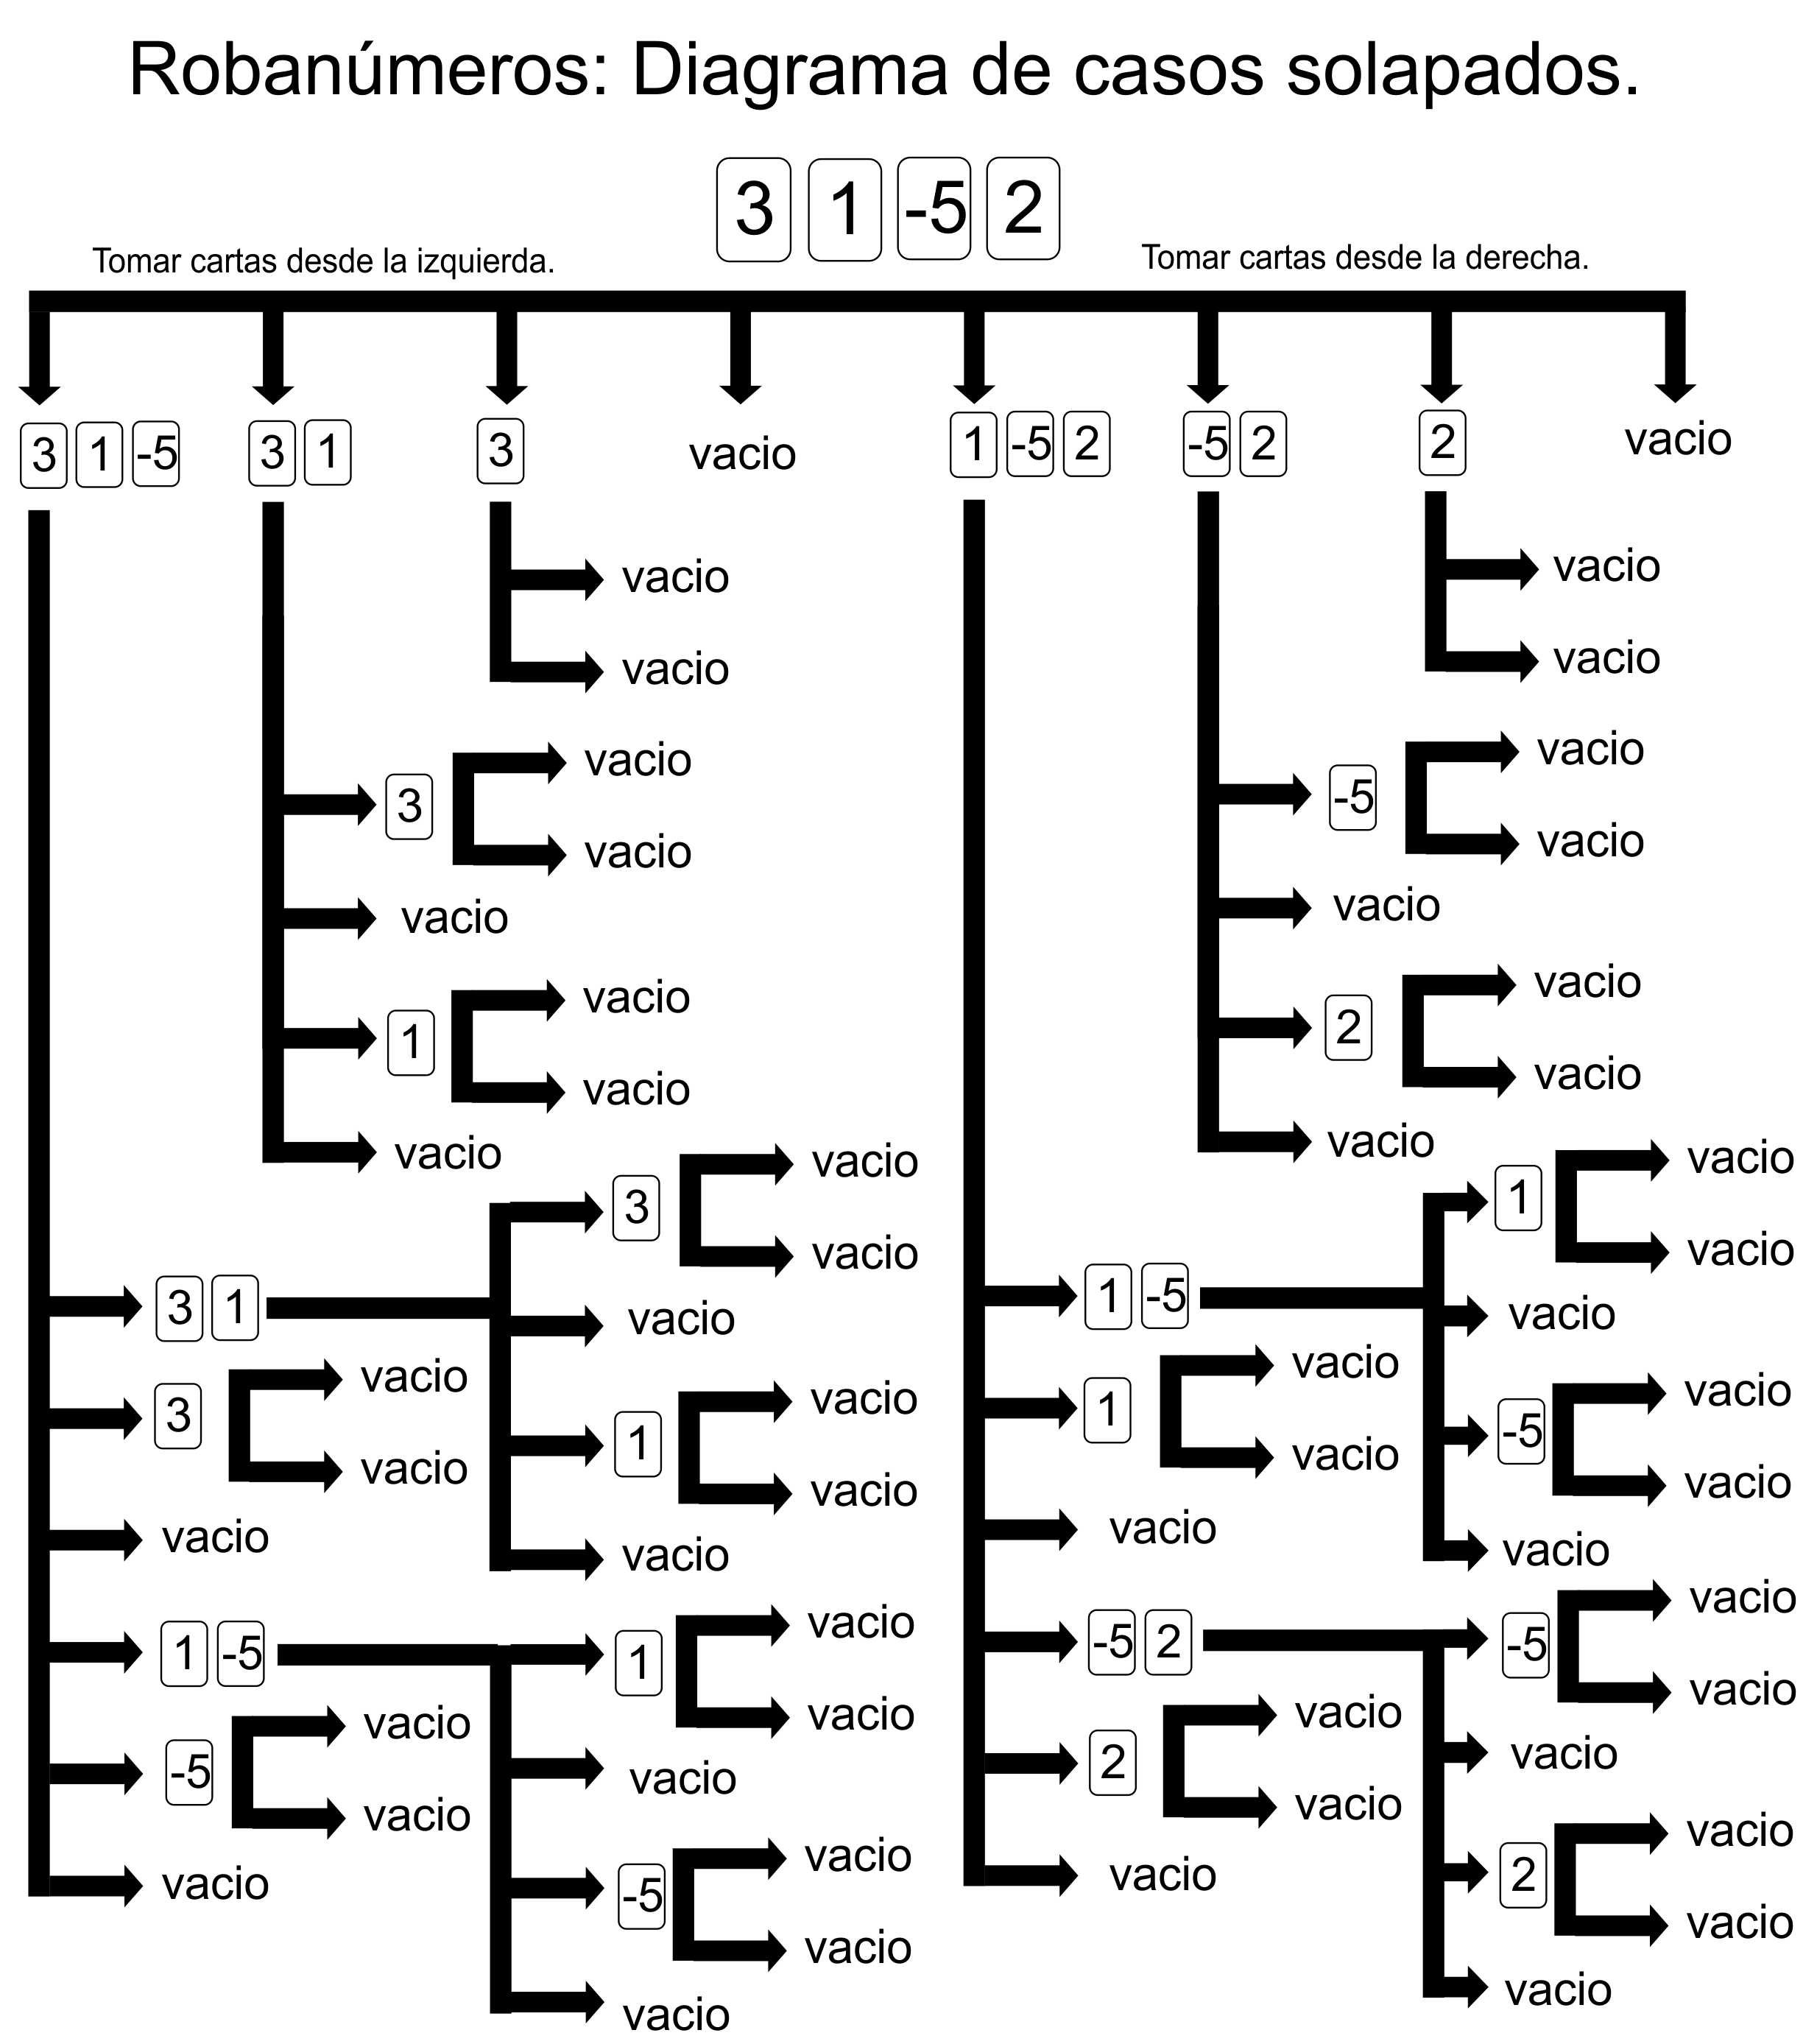
\includegraphics[width=0.8\textwidth]{ej}
  \label{fig:ejemplo}
\end{figure}
Para resolverlo creamos una matriz de (n+1)*(n+1) (siendo n la cantidad de cartas), donde almacenamos los juegos �ptimos, para
cada posible subjuego.

Establecemos como casos base el subjuego vac�o y todos los subjuegos con una carta. Luego consideramos subjuegos con una
carta m�s que el subjuego anterior, basando la soluci�n en tomar k cartas de alguno de los
extremos, y jugar de manera �ptima el subjuego resultante. En el �ltimo paso de este proceso, tenemos almacenada en la
posici�n [1,n+1] la soluci�n �ptima para el juego de n cartas.

\subsection{Correctitud}

\subsubsection{Lema 1: Principio de optimalidad}

Demostraci�n de que las soluciones de este problema cumplen el principio de optimalidad.\\

Sea Xs una soluci�n �ptima de un escenario de n cartas, donde  Xs = [$j_i$ = ($cantidad_i$, $lado_i$)], con k jugadas, entonces obtenemos la 
descomposici�n 
del juego: $j_1$ $j_2$  .. $j_k$. Cuyo resultado es Puntaje(J1)-Puntaje(J2), es decir: \\

Diferencia($1^{er}$ Jugador) = $ \sum_{i=1}^{k}{(-1)}^{i+1}Puntaje(j_{i})$\\

Luego, queremos ver que cada soluci�n esta conformada por subsoluciones �ptimas. Tomemos las dos primeras jugadas 
de Xs y descart�moslas, junto con las cartas que retiro en cada jugada. 
Llamemos a este nuevo escenario P. Estas corresponden a una jugada del jugador 1 y a una del 2  
respectivamente, porque lo que volvemos a obtener un juego donde el jugador 1 busca 
maximizar la diferencia. Sea Ys: $j'_1$ $j'_2$  .. $j'_m$ una soluci�n �ptima, para este nuevo problema de 
$n - cantidad_1 - cantidad_2$ cartas. Queremos ver que:\\

$ \sum_{i=1}^{m}{(-1)}^{i+1}Puntaje(j'_{i})$ == $ \sum_{i=3}^{k}{(-1)}^{i+1}Puntaje(j_{i})$ \\

Es decir, que $Xs - j_1 - j_2$ es una soluci�n �ptima para este subproblema P. Asumamos que no lo es: \\
Si es menor: Entonces la soluci�n dada por $Xs - j_1 - j_2$ es estrictamente mejor. Pero esto no puede ser pues supusimos Ys �ptima. \\
Si es mayor: Entonces puedo crear Xs' = $j_1$ $j_2$ Ys que es una soluci�n estrictamente mejor que Xs para el problema original, lo cual es
absurdo pues supusimos Xs �ptima. \\

Luego $Xs - j_1 - j_2$ es una soluci�n �ptima para el subproblema P.\\

Ahora descartemos solo $j_1$. Queremos ver que $Xs - j_1$ nos da la soluci�n a un subproblema T de $ n - cantidad_1$ cartas. 
Pero debemos tener en cuanta que en este subproblema, el primer 
jugador en realizar una jugada es 2, por lo tanto, la diferencia entre puntajes debe estar realizada a favor de 2.
Llamemos Zs: $j''_1$ $j''_2$  .. $j''_q$ a la soluci�n �ptima para este problema. Queremos ver que:\\

$ \sum_{i=1}^{m}{(-1)}^{i+1}Puntaje(j''_{i})$ == $ \sum_{i=2}^{k}{(-1)}^{i}Puntaje(j_{i})$ \\

Es decir, que $Xs - j_1$ es una soluci�n �ptima para este subproblema T. N�tese que debemos cambiar el signo de los t�rminos pues
antes debemos calcular Puntaje(J2)-Puntaje(J1).
Asumamos que no lo es: \\
Si es menor: Entonces la soluci�n dada por $Xs - j_1$ es estrictamente mejor. Pero esto no puede ser pues supusimos Zs optima. \\
Si es mayor: Entonces puedo crear Xs' = $j_1$ Zs que es una soluci�n en la que el jugador 2 juega estrictamente mejor que en Xs para 
el problema original, lo cual es absurdo pues supusimos Xs �ptima, y en
una soluci�n �ptima, ambos jugadores deben jugar de manera �ptima. \\

Luego $Xs - j_1$ es una soluci�n �ptima para el subproblema T.\\

Con esto, hemos demostrado que se cumple el principio de optimalidad.\\

\subsubsection{Funci�n Recursiva}

Definici�n de la funci�n que devuelve la soluci�n �ptima, donde por soluci�n nos referimos solamente a la diferencia de puntajes y no
al juego en s�,
pues almacenaremos esta informaci�n dentro del programa y no de la funci�n. \\

Sea para $|C| \geq n \geq 0$, C la secuencia de las cartas, $\Rightarrow \\
f(n, C)= \left\{ \begin{array}{lcc}
             0 &   si  & n == 0 \\
             \\C_1 &   si  & n == 1 \\
             \\ max_{1\leq i \leq n}(SI(i, C) - f(n-i, C_{[i+1..n]}), SD(i,C) - f(n-i, C_{[1..n-i]})) &  c/c &  \
             \end{array}
   \right.$\\
Donde: \\
$ SI(m, c) =  \sum_{i=1}^{m}C_{i}$ y $ SD(m,c) =  \sum_{j=|C|}^{|C|-m+1}C_{j}$ \\\\  
Sobre esta funci�n deben tenerse en cuenta varias cosas. La primera, es que el $max_{1\leq i \leq n}$ al que hacemos referencia no esta tomando 
solo dos par�metros y devolviendo el mayor, sino que para cada incide i crea un par de par�metros, y luego devuelve el m�ximo entre esos 
$2n$ par�metros.
La segunda, es que esta funci�n se indexa desde $1$ cosa que no pasa en C++. Lo hacemos de as� pues resulta mas natural y legible en un
modelo matem�tico como este, luego el pasaje a �ndices en C++ es absolutamente trivial (solo implica restar uno a todos los �ndices). Por ultimo, 
queremos notar que, si bien $C_{[i+1.. n]}$ puede indefinirse en el caso $i==n$, la funci�n f, que es llamada con el par�metro $n-i$ (que
vale $0$ en el 
caso $i==n$), esta bien definida, pues no depende de C.

\subsubsection{Lema 2: Demostraci�n de correctitud de f}

Ahora nos enfocamos en probar la correctitud de f, refiri�ndonos al hecho de que f, efectivamente devuelve la soluci�n �ptima. Para esto, 
usaremos inducci�n en la cantidad de cartas. Sea C el arreglo original de cartas, n el tama�o de C y considerando como hip�tesis 
inductiva: f devuelve la soluci�n �ptima para todo juego con menos de n cartas $\Rightarrow$

\paragraph{Caso Base:}
Consideramos dos posibles casos base, $n==0$ y $n==1$. Esto es porque ambas llamadas pueden suceder en la recursi�n, pero tienen distintos 
comportamientos.

Si $n==0$ entonces no hay cartas sobre la mesa, luego, ninguno de los jugadores tiene forma de conseguir un puntaje distinto a cero. Entonces, 
f devuelve la soluci�n �ptima en este caso, en particular, porque solo existe una soluci�n.
De la misma forma, si $n==1$ significa que solo hay una carta sobre la mesa, por lo que solo hay una soluci�n (tomar dicha carta). Luego la
soluci�n �ptima es la �nica soluci�n posible, que es $C_1$. Luego, f tambi�n devuelve la soluci�n �ptima en este caso. 

\paragraph{Paso Inductivo:}
Como hemos demostrado en 1.1.1 (principio de optimalidad), la soluci�n �ptima est� compuesta de subsoluciones �ptimas, donde llamamos
subsoluciones
a las soluciones de los posibles subjuegos. Luego, la soluci�n �ptima nunca va a estar formada por 
agarrar k cartas de alg�n modo y jugar de manera sub�ptima el resto del juego. Por lo tanto, ni siquiera nos detendremos a considerar estos 
casos como posibles soluciones.

Dicho esto, consideramos todas las dem�s posibilidades, es decir, aquellas que se forman de tomar k cartas de alguna manera y luego jugar de 
manera �ptima. O lo que es lo mismo $ \sum_{i=1}^{k}C_{i} - f(n-i, C_{[i+1..n]})$ tomando cartas desde la izquierda o
$\sum_{j=|C|}^{|C|-k}C_{j} - f(n-i, CS_{[1..n-i]}) $ tomando cartas desde la derecha.

Sabemos que la soluci�n �ptima debe ser una de estas, por lo argumentado anteriormente. Entonces, obtenemos la funci�n �ptima 
como el m�ximo de todas las posibles soluciones. Es decir:\\
$max_{1\leq k \leq n}( \sum_{i=1}^{k}C_{i}  - f(n-i, C_{[i+1..n]}), \sum_{j=|C|}^{|C|-k}C_{j} - f(n-i, CS_{[1..n-i]})) $ 
que es exactamente lo que calcula f $\forall n \geq 2$, pues por HI sabemos que f devuelve la soluci�n �ptima para todo 
juego con menos de n cartas, en particular para $n-i$ con $ 1\leq i\leq n$.

\paragraph{Conclusi�n:}Luego, f devuelve la soluci�n �ptima $\forall n$, entonces f es correcta.

\subsubsection{Lema 3: Demostraci�n de correctitud del c�digo}

Ahora nos enfocamos en probar la correctitud del c�digo P, es decir, que el c�digo efectivamente implementa f. Para esto, 
usaremos inducci�n en n, donde n es la cantidad de cartas. Sea C=cartasEnLaMesa el arreglo original de cartas, n=cantCartas el
tama�o de C y considerando como hip�tesis 
inductiva: P(k) devuelve f(k)  para toda secuencia de k cartas con $0\leq k \leq n$ $\Rightarrow$

\paragraph{Caso Base:}
Consideramos dos posibles casos base, $n==0$ y $n==1$, porque son los casos bases de f.

Si $n==0$ $\Rightarrow$ f(n, [])=0, luego, cuando n==0 en P no se ejecuta ning�n for, y devuelve \\
$jugadasOptimas[1][cantCartas]== \\
jugadasOptimas[1][n]==\\ 
jugadasOptimas[1][0] == 0 $ por la linea\\
   ($\forall 0\leq i\leq n-1$)jugadasOptimas[i][1] $\leftarrow$ 0.
   
   
De la misma forma, si $n==1$ $\Rightarrow$ f(1,[$C_1$])=$C_1$ tampoco se ejecuta ning�n for, y P devuelve \\
$jugadasOptimas[1][cantCartas]== \\
jugadasOptimas[1][n]==\\ 
jugadasOptimas[1][1] == 0 $ por la linea\\
   ($\forall 0\leq i\leq n-1$)jugadasOptimas[i][1] $\leftarrow$ 0.

\paragraph{Paso Inductivo:}
Queremos ver que P(n) devuelve f(n,C), sabemos que n$\geq 2$, por lo que P ingresa en los for's $\Rightarrow$ P devuelve\\
$jugadasOptimas[1][cantCartas]==\\
jugadasOptimas[1][n]==$\\ 
(que por linea: jugadasOptimas[comienzoSubjuego][tama�oSubjuego] $\leftarrow$ m�ximo seg�n puntaje de listaDeJugadas es)\\
== m�ximo seg�n puntaje de listaDeJugadas==\\
$max_{0\leq k \leq n}(\sum_{i=1}^{m}C_{i} - jugadasOptimas[cantCartas-k][k],\sum_{j=|C|}^{|C|-m+1}C_{j} - jugadasOptimas[cantCartas-k][0])==$\\
(por hip�tesis inductiva)  \\
==$max_{0\leq k \leq n}(\sum_{i=1}^{m}C_{i} - f(n-k, C_{[0,n-k]}),\sum_{j=|C|}^{|C|-m+1}C_{j} - f(n-k, C_{[k,n]}))==$\\
f(n, C)\\ 

Que es lo que queremos probar.
\\ \\ \textbf{Pseudoc�digo:}\\
\begin{algoritmo}{Robanumeros}{Lista<Carta> cartasEnLaMesa, Nat cantCartas}[int Puntaje]
  matriz<puntaje, jugadas> jugadasOptimas[cantCartas+1][cantCartas+1] \;
  Inicializar JugadasOptimas En Cero \;   
   ($\forall 0\leq i\leq n-1$)jugadasOptimas[i][0] \asignar 0 \;
  ($\forall 0\leq i\leq n-1$) jugadasOptimas[i][1] \asignar $C_{i}$ 
  Lista<puntaje, jugadas> listaDeJugadas \;  
  \For(){\Forcond{tama�oSubjuego \asignar 2}{cantCartas}}{      
    \For(){\Forcond{comienzoSubjuego \asignar 0}{cantCartas-tama�oSubjuego}}{      
      \For(){\Forcond{k \asignar comienzoSubjuego}{tama�oSubjuego+comienzoSubjuego}}{      
	jugada1 = $\sum_{i=1}^{m}C_{i}$ - jugadasOptimas[cantCartas-k][k] \;
	jugada2 = $\sum_{j=|C|}^{|C|-m+1}C_{j}$ - jugadasOptimas[cantCartas-k][0] \;	
	Agregar(listaDeJugadas, jugada1, jugada2) \;	
      }      
      jugadasOptimas[comienzoSubjuego][tama�oSubjuego] \asignar m�ximo seg�n puntaje de listaDeJugadas \;      
    }    
    return jugadasOptimas[1][cantCartas]     
  }
 \end{algoritmo}
 
 
\subsubsection{Conclusi�n}

Ahora sabemos, por Lema 2, que f es correcta y que, por Lema 3, P implementa f. Luego, P me devuelve la soluci�n �ptima. 

\subsection{Complejidad}

A continuaci�n vamos a analizar la complejidad temporal de las funciones relevantes del problema. Como todas estas funciones
son iterativas, las complejidades finales, que aparecen al final de cada una, son la suma de las complejidades de cada l�nea, que aparecen al
costado de las mismas.


\begin{algoritmo}{Robanumeros}{\In{cartasEnLaMesa}{List<int>},\In{n}{int}}
\LinesNumbered
\nl
\
 bool esElTurnoDelJugador1 \asignar true\tcc*{$O$(1)} \
 bool hayCartasEnLaMesa \asignar true\tcc*{$O$(1)} \
 int cantTurnos \asignar 0\tcc*{$O$(1)} \
 int inicioSubsecuenciaDeCartas \asignar 1\tcc*{$O$(1)} \
 int finSubsecuenciaDeCartas \asignar n\tcc*{$O$(1)} \
 MatrizOpt matrizJugadasOptimas[n+1][n+1] \asignar vacio\tcc*{$O$($n�$)} \
 \;
 \
 GenerarTodasLasJugadasOptimas(cartasEnLaMesa, matrizJugadasOptimas)\tcc*{$O$($n�$)}\;
 \
 \While(\tcc*[f]{$O$($n�$)}){hayCartasEnLaMesa}{
    
    \uIf(\tcc*[f]{$O$(1)}){esElTurnoDelJugador1}{

       RealizarJugadaOptimaEntre(inicioSubsecuenciaDeCartas, finSubsecuenciaDeCartas, cartasEnLaMesa, jugador1, matrizJugadasOptimas)\tcc*{$O$($n$)}

       esElTurnoDelJugador1 = false\tcc*{$O$($n�$)}
      
       }\Else{

       RealizarJugadaOptimaEntre(inicioSubsecuenciaDeCartas, finSubsecuenciaDeCartas, cartasEnLaMesa, jugador2, matrizJugadasOptimas)\tcc*{$O$($n$)}

       esElTurnoDelJugador1 = true\tcc*{$O$($1$)}

       }
       
       cantTurnos++\tcc*{$O$($1$)}
       
       hayCartasEnLaMesa = (cartasEnLaMesa.size() != 0)\tcc*{$O$($1$)}
       
    }
    \;
    return cantTurnos\tcc*{$O$($1$)} \
    \;
    Complejidad Total: $O$($n�$ + $n�$) = $O$($n�$)

 
\end{algoritmo}




\begin{algoritmo}{RealizarJugadaOptimaEntre}{\Inout{inicioSubsecuenciaDeCartas}{int}, \Inout{finSubsecuenciaDeCartas}{int}, \Inout{cartasEnLaMesa}{list<int>}, \Inout{jugador}{Jugador}, \Inout{matrizJugadasOptimas}{MatrizOpt}}
\LinesNumbered
\nl
\
 Jugada jugada \asignar ObtenerMejorJugadaEntre(inicioSubsecuenciaDeCartas, finSubsecuenciaDeCartas, matrizJugadasOptimas)\tcc*{$O$($1$)}
 string extremoDeDondeSaco \asignar jugada.first\tcc*{$O$($1$)} 
 int cantCartasQueSaco \asignar jugada.second\tcc*{$O$($1$)}
 \uIf(\tcc*[f]{$O$($1$)}){extremoDeDondeSaco == izq}{
   inicioSubsecuenciaDeCartas += cantCartasQueSaco\tcc*{$O$($1$)}
   }\Else{
   finSubsecuenciaDeCartas -= cantCartasQueSaco\tcc*{$O$($1$)}
  }
  jugador.AgregarJugada(jugada)\tcc*{$O$($1$)}
  ActualizarPuntajeJugador(cartasEnLaMesa, jugador, jugada)\tcc*{$O$($n$)}
  \;
  Complejidad Total: $O$($n$)

\end{algoritmo}


\begin{algoritmo}{ObtenerMejorJugadaEntre}{\In{inicioSubsecuenciaDeCartas}{int}, \In{finSubsecuenciaDeCartas}{int}, \Inout{matrizJugadasOptimas}{MatrizOpt}}[Jugada]
\LinesNumbered
\nl
  return matrizJugadasOptimas[inicioSubsecuenciaDeCartas][finSubsecuenciaDeCartas].second\tcc*{$O$($1$)}
  \;
  Complejidad Total: $O$($1$)

\end{algoritmo}


\begin{algoritmo}{ActualizarPuntajeJugador}{\Inout{cartasEnLaMesa}{list<int>}, \Inout{jugador}{Jugador}, \In{jugada}{Jugada}}
\LinesNumbered
\nl
 string extremoDeDondeSaco \asignar jugada.first\tcc*{$O$($1$)}
 int cantCartasARemover \asignar jugada.second\tcc*{$O$($1$)}
 int puntos\tcc*{$O$($1$)}
 \For(\tcc*[f]{$O$($|cartasEnLaMesa|$) = $O$($n$)}){\Forcond{cantCartas \asignar 0}{cantCartasARemover}}{
 \uIf(\tcc*[f]{$O$($1$)}){extremoDeDondeSaco == izq}{
  puntos \asignar cartasEnLaMesa.front()\tcc*{$O$($1$)}
  cartasEnLaMesa.popFront()\tcc*{$O$($1$)}
 }\Else{
  puntos \asignar cartasEnLaMesa.back()\tcc*{$O$($1$)}
  cartasEnLaMesa.popBack()\tcc*{$O$($1$)}
 }
 jugador.AgregarPuntos(puntos)\tcc*{$O$($1$)}
}\;

Complejidad Total: $O$($n$)


\end{algoritmo}



\begin{algoritmo}{GenerarTodasLasJugadasOptimas}{\Inout{listaDeCartas}{list<int>}, \Inout{matrizJugadasOptimas}{MatrizOpt}}
\LinesNumbered
\nl
 int n \asignar listaDeCartas.size()\tcc*{$O$($1$)}
 vector<int> cartasEnLaMesa[n+1]\tcc*{$O$($n$)}
 //Paso todas las cartas de una lista a un vector, porque me es mas conveniente para las demas funciones.\;
 PasarDeListaAVector(cartasEnLaMesa, listaDeCartas)\tcc*{$O$($n$)}
 //Lleno la diagonal con los casos base\;
 GenerarCasosBase(cartasEnLaMesa, matrizJugadasOptimas)\tcc*{$O$($n$)} 
 GenerarElRestoDeLosCasos(cartasEnLaMesa, matrizJugadasOptimas)\tcc*{$O$($n�$)}\;
 
 Complejidad Total: $O$($n�$)

\end{algoritmo}


\begin{algoritmo}{GenerarElRestoDeLosCasos}{\Inout{cartasEnLaMesa}{vector<int>}, \Inout{matrizJugadasOptimas}{MatrizOpt}}
\LinesNumbered
\nl
 int n \asignar cartasEnLaMesa.size() - 1\tcc*{$O$($1$)}

  //Lleno la matriz de abajo para arriba, de izquierda a derecha\;
  \For(\tcc*[f]{$O$($n�$)}){\Forcond{inicioSubsecuenciaDeCartas \asignar n-1}{1}}{
      \For(\tcc*[f]{$O$($n�$)}){\Forcond{finSubsecuenciaDeCartas \asignar inicioSubsecuenciaDeCartas+1}{n}}{
        //ObtenerSumaIzquierdaDeLasCartasEntre calcula $\sum_{i=inicioSubsecuenciaDeCartas}^{finSubsecuenciaDeCartas}cartasEnLaMesa_{i}$\;
        //ObtenerSumaDerechaDeLasCartasEntre calcula $\sum_{j=finSubsecuenciaDeCartas}^{inicioSubsecuenciaDeCartas}cartasEnLaMesa_{j}$\;
        \;
         vector<int> sumaParcialIzquierda \asignar ObtenerSumaIzquierdaDeLasCartasEntre(inicioSubsecuenciaDeCartas, finSubsecuenciaDeCartas, cartasEnLaMesa)\tcc*{$O$($n$)} 
         vector<int> sumaParcialDerecha \asignar ObtenerSumaDerechaDeLasCartasEntre(inicioSubsecuenciaDeCartas, finSubsecuenciaDeCartas, cartasEnLaMesa)\tcc*{$O$($n$)}
         //JugadaOptima == < beneficio a mi favor, jugada que debo hacer >\;
         JugadaOptima jugadaOptimaIzq \asignar ObtenerJugadaOptimaDesdeLaIzquierda(sumaParcialIzquierda, inicioSubsecuenciaDeCartas, finSubsecuenciaDeCartas, matrizJugadasOptimas)\tcc*{$O$($n$)} 
         JugadaOptima jugadaOptimaDer \asignar ObtenerJugadaOptimaDesdeLaDerecha(sumaParcialDerecha, inicioSubsecuenciaDeCartas, finSubsecuenciaDeCartas, matrizJugadasOptimas)\tcc*{$O$($n$)} 
         JugadaOptima jugadaOptima\tcc*{$O$($1$)}\; 
         \uIf(\tcc*[f]{$O$($1$)}){jugadaOptimaIzq.first > jugadaOptimaDer.first}{
            jugadaOptima \asignar jugadaOptimaIzq\tcc*{$O$($1$)} 
         }\Else{
            jugadaOptima \asignar jugadaOptimaDer\tcc*{$O$($1$)} 
         }
         
         matrizJugadasOptimas[inicioSubsecuenciaDeCartas][finSubsecuenciaDeCartas] \asignar jugadaOptima\tcc*{$O$($1$)} 
         
      }

     }
     
     Complejidad Total: $O$($n�$)
     
\end{algoritmo}


\begin{algoritmo}{ObtenerJugadaOptimaDesdeLaIzquierda}{\Inout{sumaParcialIzquierda}{vector<int>}, \In{inicioSubsecuenciaDeCartas}{int}, \In{finSubsecuenciaDeCartas}{int}, \Inout{matrizJugadasOptimas}{MatrizOpt}}[JugadaOptima]
\LinesNumbered
\nl
int cantCartas \asignar sumaParcialIzquierda.size() - 1\tcc*{$O$($1$)} 
JugadaOptima jugadaOptima  //< beneficio a mi favor, jugada que debo hacer > \tcc*{$O$($1$)} 
Jugada jugada //<extremo, cant de cartas>\tcc*{$O$($1$)} 
jugada.first \asignar izq\tcc*{$O$($1$)}
int mayorBeneficioAFavor \asignar 0\tcc*{$O$($1$)} 
bool todaviaNoCalculeNingunBeneficio \asignar true\tcc*{$O$($1$)} \;

  \For(\tcc*[f]{$O$($cantCartas$) = $O$($n$)}){\Forcond{cantCartasAgarradas \asignar 1}{cantCartas}}{
      int sumaDeLasPrimerasICartas \asignar sumaParcialIzquierda[cantCartasAgarradas]\tcc*{$O$($1$)} 
      int mayorBeneficioDelOponente\tcc*{$O$($1$)} 
     
     \uIf(\tcc*[f]{$O$($1$)}){cantCartasAgarradas < cantCartas}{
	//El beneficio del oponente es lo mejor que se puede sacar de la subsecuencia de cartas restante.\;
	mayorBeneficioDelOponente \asignar matrizJugadasOptimas[inicioSubsecuenciaDeCartas+cantCartasAgarradas][finSubsecuenciaDeCartas].first\tcc*{$O$($1$)}
	}\Else{
	//Si agarre todas las cartas, el beneficio del oponente obviamente es 0.\;
	mayorBeneficioDelOponente \asignar 0\tcc*{$O$($1$)}
	}
	
	\If(\tcc*[f]{$O$($1$)}){todaviaNoCalculeNingunBeneficio}{
	    //Como todavia no tengo ningun beneficio a favor, agarro el primero que calculo y lo tomo como maximo\;
	    mayorBeneficioAFavor \asignar sumaDeLasPrimerasICartas - mayorBeneficioDelOponente\tcc*{$O$($1$)}
	    todaviaNoCalculeNingunBeneficio \asignar false\tcc*{$O$($1$)}
	}
        
        \If(\tcc*[f]{$O$($1$)}){mayorBeneficioAFavor <= sumaDeLasPrimerasICartas - mayorBeneficioDelOponente}{
	    //Actualizo cual seria mi mejor jugada\;
	    mayorBeneficioAFavor \asignar sumaDeLasPrimerasICartas - mayorBeneficioDelOponente\tcc*{$O$($1$)}
	    jugada.second \asignar cantCartasAgarradas\tcc*{$O$($1$)}
	    jugadaOptima.first \asignar mayorBeneficioAFavor\tcc*{$O$($1$)}
	    jugadaOptima.second \asignar jugada\tcc*{$O$($1$)}
	    
	 }

   }

  return jugadaOptima\tcc*{$O$($1$)}\;
  
  Complejidad Total: $O$($n$)


\end{algoritmo}


ObtenerJugadaOptimaDesdeLaDerecha es igual a la anterior, con la diferencia de que la l�nea 9 se reemplaza por:
\newline
int sumaDeLasPrimerasICartas = sumaParcialDerecha[cantCartasAgarradas]
\newline
y la linea 13 es reemplazada por: 
\newline
mayorBeneficioDelOponente = matrizJugadasOptimas[inicioSubsecuenciaDeCartas][finSubsecuenciaDeCartas-cantCartasAgarradas].first

 


\subsection{Testing}
Los casos bordes que consideramos en este ejercicio son los que tienen una sola carta, todas las cartas positivas,
y todas negativas. Para ello, usamos las siguientes entradas.
\begin{center}
  \begin{tabular}{| l | c | r | c | r | c | r | c | r | }
    \hline
     Cantidad de cartas & Cartas & Turnos & Puntajes J1 J2 & Jugadas \\ \hline
     1 & [1] & 1 & J1=1 J2=0 & izq 1 \\ \hline
     4 & [3,2,25,62] & 1 & J1=92 J2=0 & der 4 \\ \hline
     4 & [-1,-1,-1,-500] & 2 & J1=-3 J2=-500 & izq 3 izq 1 \\ 
     \hline
   \end{tabular}
 \end{center}
 N�tese que en el caso en el cual todas las cartas son negativas la soluci�n no es trivial ni �nica. Pero aun as� lo consideramos como un 
 caso borde
 pues el algoritmo podr�a, si estuviese mal implementado, maximizar la ganancia sin tener en cuenta futuras p�rdidas si bien no es el caso.
\paragraph{Nota}
La validez de estos resultados se comprob� a mano, mas no se adjuntan las cuentas pues creemos que no aportan mucho m�s que espacio
malgastado. (Salvemos un �rbol! Ahorremos papel!)


\subsection{Experimentaci�n}

\subsubsection{Generaci�n de Tests Aleatorios}

Para generar los tests aleatorios, utilizamos el siguiente c�digo:

\begin{verbatim}
 
 
    int main() {

        srand(time(NULL));
        ofstream tests;
        tests.open("tests_aleatorios");
        int MAX_CARTAS = 1000;

        for (int maximoDeCartas = 1; maximoDeCartas <= MAX_CARTAS; maximoDeCartas+=25) {

        tests << maximoDeCartas << " ";

        for (int cantCartas = 1; cantCartas <= maximoDeCartas; cantCartas++) {

            int nroRandom = 2*(rand() % maximoDeCartas + 1);
            int carta = nroRandom - maximoDeCartas;
            tests << carta << " ";
            
            }
            
            tests << endl;
            
        }
        
        tests << 0;
        tests.close();

    }

\end{verbatim}


Utilizamos la hora del reloj de la computadora al momento de la ejecuci�n como semilla para la funci�n rand(). Por conveniencia, 
los n�meros de las cartas
se mueven entre -n y n, es decir, tanto el m�nimo como el m�ximo n�mero est�n en O(n), siendo n la cantidad de cartas sobre la mesa.


\subsubsection{Gr�ficos}

A la hora de graficar, decidimos comparar un caso ``general'', es decir, con tanto n�meros positivos como negativos generados aleatoriamente, contra casos borde como por ejemplo todos n�meros positivos, y todos
n�meros negativos. A continuaci�n se pueden observar los resultados:

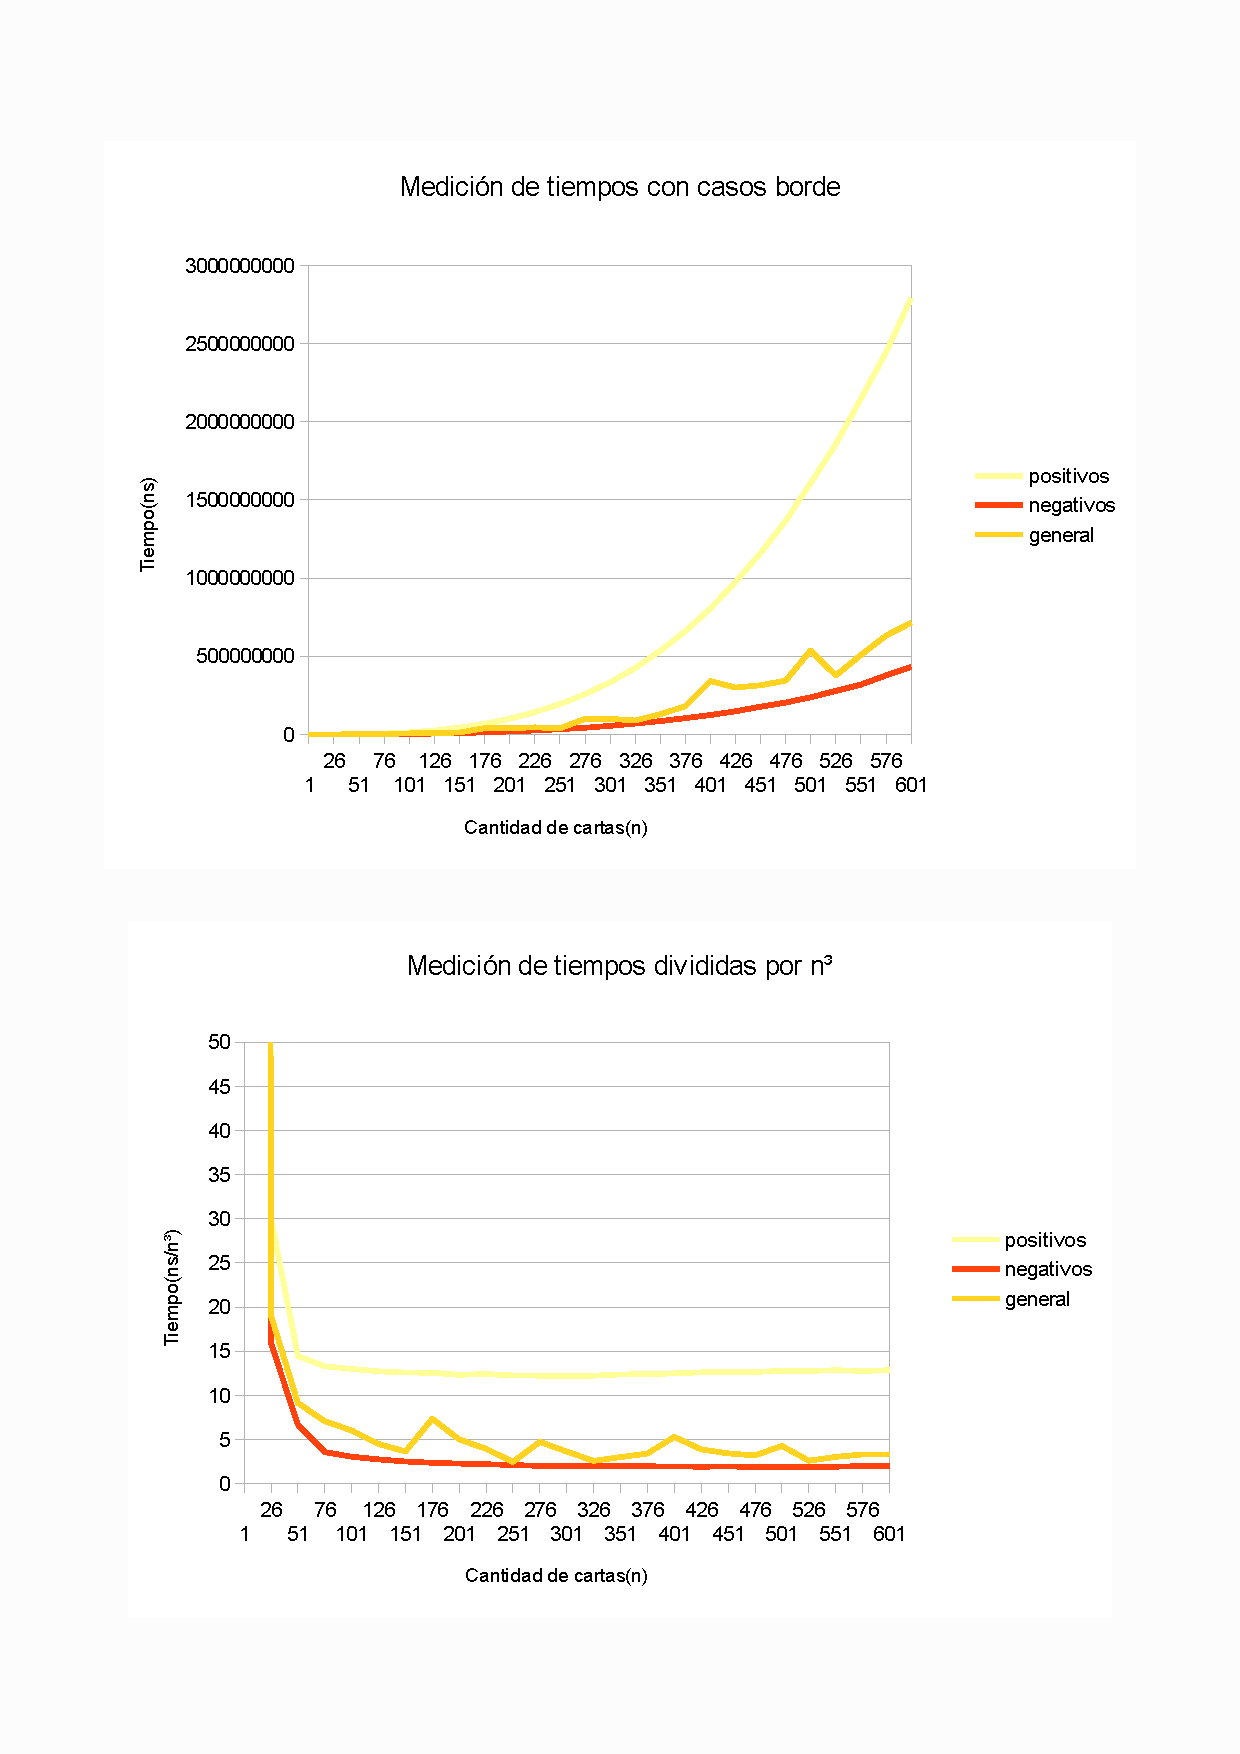
\includegraphics[width=0.8\textwidth]{ej1/graficos.pdf}

\subsubsection{Conclusiones}

Lo que pudimos observar emp�ricamente fue que, a diferencia de lo que intuitivamente pensamos, los casos donde todas las cartas son positivas son los casos que m�s tiempo toman, mientras que los casos donde todas las
cartas son negativas, son los que menos tiempo toman.
En el segundo gr�fico tambi�n pudimos corroborar emp�ricamente que los tiempos de ejecuci�n crecen como una funci�n c�bica del tama�o de la entrada, ya que al dividir los tiempos de ejecuci�n por $n�$, los mismos tienden a 
un n�mero constante.

%\newpage
%\section{Problema 2: La centralita (de gas)}

%\subsection{Descripcion del problema}
El problema consiste en, dada:\\

-Una lista con $n$ pueblos, representados con sus pociciones $x$ e $y$ en el plano.\\

-Un numero $k$ que representa la cantidad maxima de centrales de gas a construir.\\

Conectar todos los pueblos a la red de gas construyendo centrales en a lo sumo pueblos y conectandolos por tuberias al resto de los pueblos, intentando minimizar el $riesgo$. donde el $riesgo$ es la distancia maxima de una tuberia construida entre dos pueblos.\\

Abstrayendonos del problema, podemos ver a los pueblos y tuberias como vertices y aristas de un grafo, y lo que queremos lograr es conseguir a lo sumo $k$ componentes conexas tales que el peso maximo entre todas las aristas sea minimo.

\subsubsection{Ejemplos}
Sea N el numero de pueblos, K la cantidad maxima de centrales, Pos:lista<ParXY> las posiciones de los pueblos en el plano, Q la cantidad de centrales construidas, M la cantidad de tuberias construidas, Centrales:lista<pueblos> los pueblos con centrales en ellos y Conexiones:lista<ParPueblo1Pueblo2> los vertices de las tuberias construidas (vease que una tuberia con vertices $x$ e $y$ es lo mismo que una tuberia con vertices $y$ y $x$).$\Rightarrow$
\begin{enumerate}
\item N: 1, K: 1, Pos:{(0,0)} \\
la respuesta es unica:
\begin{center}
  
   \begin{tabular}{| l | c | r | c | r | c | r | }
     \hline
     Q & M & Centrales & Conexiones \\ \hline
     1 & 0 & [1] & [ ]  \\
     \hline
   \end{tabular}
\end{center}

\item N: 2, K: 1, Pos:{(0,0),(0,1)} \\
las respuestas posibles son:
\begin{center}
  
   \begin{tabular}{| l | c | r | c | r | c | r | }
     \hline
     Q & M & Centrales & Conexiones \\ \hline
     1 & 1 & [1] & [(1,2)]  \\ \hline
     1 & 1 & [2] & [(1,2)] \\ 
     \hline
   \end{tabular}
 \end{center}
 
Vease que la central puede ubicarse tanto en un pueblo como en el otro.

\item N: 3, K: 2, Pos:{(0,0),(0,1),(8,8)} \\
las respuestas posibles son:
\begin{center}
  
   \begin{tabular}{| l | c | r | c | r | c | r | }
     \hline
     Q & M & Centrales & Conexiones \\ \hline
     1 & 1 & [1,3] & [(1,2)]  \\ \hline
     1 & 1 & [2,3] & [(1,2)] \\ 
     \hline
   \end{tabular}
 \end{center}
Como el pueblo agregado esta lejos de los otros y K=2 entonces tendra su propia central
\end{enumerate}

\subsection{Resolucion}
Para la resolucion de este problema lo primero que hicimos fue buscar como conectar todas los vertices como si solo tuvieramos una estacion, al hacerlo nos dimos cuenta de que podiamos usar prim sobre una tabla de adyacencias que tuviera todas las distancias entre pueblos. hacer prim nos servia, pues por el Lema 1, demostrado mas abajo, que dice que si minimizamos la suma de los pesos del arbol $\Rightarrow$ el peso maximo entre todas las aristas es minimo, tendriamos un arbol que cumplia que el peso maximo era minimo.
Luego teniamos que lograr esto para cuando hubiera mas de una estacion, asi llegamos al Lema 2, que dice que si a un arbol minimo le quitamos su mayor elemento $\Rightarrow$ las componentes conexas resultantes forman un bosque tal que el peso maximo entre todas las aristas sea minimo. asi que quitandole las k-1 aristas maximas al arbol minimo conceguiriamos un bosque de k componentes conexas que cumplian esta propiedad.
Finalmente faltaba ver donde poner las estaciones para que cada componente conexa del bosque tenga una y solo una estacion. vimos que poner la estacion en cualquier pueblo de una componente conexa no cambiaba las aristas del resultado. asi que recorrimos el bosque poniendo una estacion en cada componente conexa.

\subsubsection{Pseudocodigo}
\begin{algoritmo}{resolver}{\In{nPueblos}{Nat}, \In{kCentrales}{Nat}, \In{pueblos}{Lista<Coordenadas>}}
	Matrix tablaDistancias(nPueblos) \;
	tablaDistancias.llenarDistancias(nPueblos,pueblos) \;
	Lista(Par(Arista,double)) arbolMinimo \;
	Lista(Par(Arista,double)) bosqueMinimo \;
	\For{Nat \asignar 1 ; i $\leq$ nPueblos ; i++}{
		Nat j \asignar tablaDistancias.MinimoFila0()\;
		double distancia = tablaDistancias.DistanciaDe(0,j)\;
		Nat origen = tablaDistancias.OrigenDe(0,j)\;
		arbolMinimo.pushfront((origen,j),distancia)\;
		tablaDistancias.Combinar(j)
	}\;
	\If {kCentrales > nPueblos}{
		kCentrales = nPueblos\;
	}
	bosqueMinimo \asignar quitarKMasGrandes(arbolMinimo,kCentrales-1) \;
	Nat cantidadTuberias = bosqueMinimo.size() \;
	List(Nat) estaciones = generarEstaciones(bosqueMin,nPueblos) \;
	devolver(kCentrales, cantidadTuberias , estaciones, bosqueMinimo) \;
	
\end{algoritmo}

\subsection{Correctitud}
\subsubsection{Idea}
Sea $\Omega$ el grafo en el que los vertices representan los pueblos y las aristas las conexiones de gas posibles entre los pueblos con su riesgo, queremos demostrar que existe un arbol generador tal que el peso maximo entre las aristas es minimo. Como $\Omega$ es conexo, pues cada pueblo se conecta con todos los otros pueblos, sabemos que existe un $\Pi$ arbol generador minimo tal que se minimize la suma de los pesos del arbol. Por el Lema 1, como existe $\Pi$ puedo encontrar $\Pi'$ un arbol generador tal que el peso maximo entre las aristas es minimo.\\
luego queremos ver que quitarle aristas me devuelve un bosque correcto, por el Lema 2 cada vez que a un arbol de minimo maximo le quito su arista mas grande genero un bosque de minimo Maximo. Por lo tanto como quitamos las aristas mas grandes del bosque, y nunca sacamos mas que la cantidad de aristas que tiene el bosque, tenemos un bosque de minimo maximo. \\
Por ultimo queremos ver que genero una estacion y solo una en cada componente conexa del bosque, lo que hacemos es poner una en un vertice y recorrer todo el arbol del que es parte, y solo pongo estaciones en vertices que no recorri, cuando todos los vertices fueron recorridos se que hay una estacion en cada componente y se que es unica porque nunca recorro mas de una vez el mismo arbol.



\subsubsection{Lema 1: AGM $\Rightarrow$ peso maximo entre aristas minimo}
Sea $T$ un AGM del grafo $\Omega$, vease que:\\

$Peso(T) = \sum_{e \in T} Peso(e)$\\

$Peso(T) \leq Peso(T') \forall T'$ arbol generador de $\Omega$\\

llamo max(T) al maximo eje entre todos los ejes de T \\

Quiero ver que:\\

$Peso(T) \leq Peso(T') \forall T'$ arbol generador de $\Omega \Rightarrow$ max(T) $\leq$ max(T')\\

supongo que tengo un T' Arbol generador de G tal que max(T') < max(T) $\Rightarrow$ $\exists$ a arista, a $\in$ T, a $\notin$ T' que conecta dos vertices x e y, si sacaramos este vertice tendriamos dos componentes conexas que llamare A y B.\\

$\exists$ a' $\in$ T' / a' va de un nodo de A a un nodo de B (si este nodo no existiera T' no seria conexo). tomo:\\

T* = T - a + a'\\

$Peso(T$*$) = \sum_{e \in T} Peso(e) - Peso(a) + Peso(a')$\\

vease que $-Peso(a) + Peso(a') < 0$ pues a es algun maximo de T y todo a' en T' es menor que a, pues max(T') < max(T)\\

Por lo tanto: $Peso(T$*$) = \sum_{e \in T} Peso(e) - Peso(a) + Peso(a') < \sum_{e \in T} Peso(e) = Peso(T)$ ABSURDO!\\

el absurdo viene de suponer que max(T') < max(T) QED.

\subsubsection{Lema 2: AGM $\Rightarrow$ B = AGM - AristaMaxima es Bosque de minimos maximos}
Sea T un AGM de $\Omega$\\

B esta dividido en dos componentes conexas X e Y\\

Supongo que B = T - AristaMaxima no es Bosque de minimos maximos del grafo $\Omega$.\\

Sea G' un Grafo de minimos maximos del grafo $\Omega$ de dos componentes conexas, se que existe pues es tomar todos las aristas ordenadas y agregarle la arista minima hasta tener 2 componentes conexas, se que existe X' e Y' subarboles AGM de cada una de sus componentes conexas, pues para que halla un AGM en un grafo solo es necesario que sea conexo. llamo B' a X'+Y', que es un Bosque de minimos maximos de dos componentes conexas.\\

Se que existe en $\Omega$ una arista de peso minimo que une X' e Y', llamo a esta arista e'. $T'$ = X'+Y'+e' es un AGM de $\Omega$.\\

peso(T') = P(X')+P(Y')+P(e')\\

peso(T) = P(X)+P(Y)+P(AristaMaxima)\\

Vease que peso(T)=peso(T') pues ambos son AGM\\

si peso(e') $\leq$ peso(AristaMaxima) $\Rightarrow$ peso(X')+peso(Y') $\geq$ peso(X)+peso(Y) absurdo pues B es bosque minimo maximo y B' no\\

si peso(e') > peso(AristaMaxima) $\Rightarrow$ peso(X')+peso(Y') = peso(X)+peso(Y) absurdo T' no puede ser arbol minimo pues max(T') > max(T) 


\subsubsection{Conclusion}
Ahora sabemos que podemos encontrar un bosque de minimo maximo para cualquier conjunto de pueblos y podemos devolver un vertice de cada arbol del bosque.

\subsection{Complejidad}

\subsubsection{Introduccion}

Puede comprobarse en el c�digo que, omitiendo la carga de datos y las iteraciones requeridas
para manejar las distintas intancias del problema, el algoritmo ejecutado para la resoluci�n del problema es el siguiente.

Debajo del algoritmo se encuentran varias aclaraciones identificadas por el n�mero de l�nea.\\
\begin{algoritmo}{resolver}{\In{nPueblos}{Nat}, \In{kCentrales}{Nat}, \In{pueblos}{Lista<Coordenadas>}}
\LinesNumbered
\nl	
	Matrix tablaDistancias(nPueblos)\tcc*{$O$($n^2$)}
	tablaDistancias.llenarDistancias(nPueblos,pueblos) \tcc*{$O$($n^2$)}
	Lista(Par(Arista,double)) arbolMinimo \tcc*{$O$(1)}
	Lista(Par(Arista,double)) bosqueMinimo \tcc*{$O$(1)}
	\For(\tcc*[f]{$O$($n^2$)}){Nat i \asignar 1 ; i $\leq$ nPueblos ; i++}{
		Nat j \asignar tablaDistancias.MinimoFila0()\tcc*{$O$($n$)}
		double distancia = tablaDistancias.DistanciaDe(0,j)\tcc*{$O$(1)}
		Nat origen = tablaDistancias.OrigenDe(0,j)\tcc*{$O$(1)}
		arbolMinimo.pushfront((origen,j),distancia)\tcc*{$O$(1)}
		tablaDistancias.Combinar(j)\tcc*{$O$($n$)}
	}
	bosqueMinimo \asignar quitarKMasGrandes(arbolMinimo,kCentrales-1) \tcc*{$O$($nlog(n)$)}
	Nat cantidadTuberias = bosqueMinimo.size() \tcc*{$O$($n$)}
	Lista(Nat) estaciones = generarEstaciones(bosqueMin,nPueblos) \tcc*{$O$($n^2$)}
	devolver(kCentrales, cantidadTuberias , estaciones, bosqueMinimo) \tcc*{$O$($n$)}
	
\end{algoritmo}

\begin{algoritmo}{llenarDistancias}{\In{nPueblos}{Nat}, \In{pueblos}{Lista<Coordenadas>}}
\LinesNumbered
\setcounter{AlgoLine}{15}
\nl	
	Lista(Coordenada)::constiterator itI = pueblos.begin()\tcc*{$O$(1)}
	list(Coordenada)::constiterator itJ = pueblos.begin()\tcc*{$O$(1)}
	\For(\tcc*[f]{$O$($n^2$)}){Nat i \asignar 0; i != nPueblos ; i++}{
		double x1 = itI->first\tcc*{$O$(1)}
		double y1 = itI->second\tcc*{$O$(1)}
		\For(\tcc*[f]{$O$(n)}){Nat f \asignar 0; f != nPueblos ; f++}{
			double x2 = itJ->first\tcc*{$O$(1)}
			double y2 = itJ->second\tcc*{$O$(1)}
			double distancia = infinito\tcc*{$O$(1)}
			\If(\tcc*[f]{$O$(1)}){i != j}{
				distancia = sqrt((x1-x2)*(x1-x2) + ((y1-y2)*(y1-y2)))\tcc*{$O$(1)}
			}
			matriz[i][j].first = distancia\tcc*{$O$(1)}
			matriz[i][j].second = i+1\tcc*{$O$(1)}
			itJ++\tcc*{$O$(1)}
		}
		itI++\tcc*{$O$(1)}
		itJ = pueblos.begin()\tcc*{$O$(1)}
	}
	
\end{algoritmo}
\begin{algoritmo}{Combinar}{\In{fila}{Nat}}
\LinesNumbered
\setcounter{AlgoLine}{34}
\nl
	Nat dimension = Columnas()\tcc*{$O$(1)}
	double inf = infinito\tcc*{$O$(1)}
	matriz[0][fila].first = inf\tcc*{$O$(1)}
	\For(\tcc*[f]{$O$(n)}) {Nat j = 0 ; j != dimension ; j++}{
		Arista aristaF1 = makepair(0,j)\tcc*{$O$(1)}
		Arista aristaF2 = makepair(fila,j)\tcc*{$O$(1)}
		\If(\tcc*[f]{$O$(1)}){esfinito(DistanciaDe(aristaF1)) and DistanciaDe(aristaF2) $<$ DistanciaDe(aristaF1)}{
			matriz[0][j].first = DistanciaDe(aristaF2)\tcc*{$O$(1)}
			matriz[0][j].second = OrigenDe(aristaF2)\tcc*{$O$(1)}
		}
	}
\end{algoritmo}
\begin{algoritmo}{generarEstaciones}{\In{bosqueMinimo}{Lista(Par(Arista,double))},\In{nPueblos}{Nat}}[Lista(Nat)]
\LinesNumbered
\setcounter{AlgoLine}{45}
\nl
	Lista(Nat) res\tcc*{$O$(1)}
	vector(bool) yaLoVi (nPueblos, false)\tcc*{$O$(n)}
	vector(bool) conectados (nPueblos, false)\tcc*{$O$(n)}
	list(Nat) proximosVer\tcc*{$O$(1)}
	\For(\tcc*[f]{$O$(n)}){Nat i=0 ; i $<$ nPueblos ; i++}{
		proximosVer.pushback(i)\tcc*{$O$(1)}
	}
	\While(\tcc*[f]{$O$($n^2$)}){!proximosVer.empty()}{
		Nat sacar = proximosVer.front()\tcc*{$O$(1)}
		\uIf(\tcc*[f]{$O$(1)}){yaLoVi[sacar]}{
			proximosVer.popfront()\tcc*{$O$(1)}
		}\Else{
			\If(\tcc*[f]{$O$(1)}){!conectados[sacar]}{
				res.pushfront(sacar+1)\tcc*{$O$(1)}
			}
			proximosVer.popfront()\tcc*{$O$(1)}
			conectados[sacar] = true\tcc*{$O$(1)}
			yaLoVi[sacar] = true\tcc*{$O$(1)}
			lista(pair(Arista,double))::iterator itAM = bosqueMinimo.begin()\tcc*{$O$(1)}
			\While(\tcc*[f]{$O$($n$)}){itAM != bosqueMinimo.end() and bosqueMinimo.size() != 0}{
				\uIf {itAM-$>$first.first == sacar}{
					Nat j = itAM-$>$first.second\tcc*{$O$(1)}
					\If(\tcc*[f]{$O$($1$)}){!conectados[j]}{
						proximosVer.pushfront(j)\tcc*{$O$(1)}
						conectados[j] = true\tcc*{$O$(1)}
					}
					itAM = bosqueMinimo.erase(itAM)\tcc*{$O$(1)}
				}\textbf{else }\uIf(\tcc*[f]{$O$(1)}){itAM-$>$first.second == sacar}{
					Nat j = itAM-$>$first.first\tcc*{$O$(1)}
					\If(\tcc*[f]{$O$(1)}){!conectados[j]}{
						proximosVer.pushfront(j)\tcc*{$O$(1)}
						conectados[j]=true\tcc*{$O$(1)}
					}
					itAM = bosqueMinimo.erase(itAM)\tcc*{$O$(1)}
				}\Else{
					itAM++\tcc*{$O$(1)}
				}
			}
		}
	}
	return res\tcc*{$O$(n)}
\end{algoritmo}
\subsubsection{Aclaraciones del Pseudoc�digo}
1) inicializar una matriz vacia de tama�o nPueblos*nPueblos tarda $O$($n^2$)\\

2) Detallado entre las lineas 16 y 34,Llenar distancias toma cada pueblo y calcula su distancia con todos los demas, esto se logra en $O$($n^2$) iteraciones.\\

5) el while se corre n-1 veces, y adentro del while hay cosas que tardan $O$($n$), asi que la complejidad es $O$($n^2$).\\

6) buscar el minimo en un arreglo de n elementos desordenados tarda $O$($n$)\\

10) Detallado entre las lineas 35 y 45, lo que hace es combinar la fila 1 con la fila indicada, lo hace recorriendo las dos filas y guardando el minimo y su origen, recorrer de esta manera las dos filas es $O$($n$)\\

12) quitarKmasGrandes ordena el arbolMinimo de distancia de arista menor a distancia de arista mayor, ordenar cuesta $O$($nlog(n)$), luego de esto quita los k elementos mas grandes pasados como parametro, como como maximo puedo quitar las n aristas esto cuesta $O$($n$). por lo tanto la complejidad total es $O$($nlog(n)$)+$O$($n$)=$O$($nlog(n)$)\\

14) Detallado entre las lineas 46 y 86, generarEstaciones devuelve exactamente un nodo de cada componente conexa.\\

47) el vector yaLoVi sirve para saber si ya busque los adyacentes de un nodo alguna vez\\

48) el vector conectados sirve para agregar los adyacentes encontrados.\\

49) proximos ver es una lista en la cual se guardan los proximos nodos a los que se le buscaran adyacentes. antes de entrar al while lo inicializo con los pueblos de 1 a n.\\

53) la cantidad de veces maxima que se correra este while es 2n, pues puedo agregar pueblos al frente de la lista solamente si no se han agregado antes, o sea si en el vector conectados estaba en false su posicion. o sea que como maximo agregare todos los pueblos al frente de la lista y cada pueblo estara dos veces en la lista, pero me aseguro de no correr la busqueda de adyacentes de un nodo que ya vi con el vector yaLoVi. como este while se corre $O$($n$) veces, y adentro hay algo que se corre $O$($n$) veces cada vez que se llama el algoritmo, entonces es $O$($n^�$)

\subsubsection{Conclusion}

Como este algoritmo es iterativo, o sea no tiene partes recursivas, la complejidad total es la suma de las complejidades, luego si sumamos las complejidades de cada linea obtenemos que este algoritmo es O($n^2$), siendo n la cantidad de pueblos del mapa. ademas, como la cantidad de centrales siempre se puede acotar por la cantidad de pueblos (una central por pueblo) en los puntos en los que la complejidad depende de la cantidad de centrales siempre la podemos acotar por la cantidad de pueblos.

\subsection{Testing}
Los casos bordes que consideramos en este ejercicio son los que:
\begin{enumerate}
\item tienen muchos pueblos en un solo lugar
\item tienen tres pueblos que estan a distancias iguales entre ellos
\item tienen mas pueblos que estaciones
\item tienen pueblos en los cuadrantes positivos y negativos del mapa

\end{enumerate}
\begin{center}
  \begin{tabular}{| l | c | r | c | r |c | r | }
    \hline
     Numero Estaciones & Pueblos & Estaciones construidas & Conexiones construidas \\ \hline
     2 & [(1,1),(1,1),(1,1)] & [1,2] & [(3,1)] \\ \hline
     2 & [(0,0),(0,10),($\sqrt{10^2-5^2}$,5)] & [1,2] & [(3,2)] \\ \hline
     100 & [(1,1),(2,2),(2,2)] & [1,2,3] & [ ] \\ \hline
     2 & [(1,1),(1,-1),(-1,1),(-1,-1)] & [1,2] & [(4,2),(3,1)] \\ 
     \hline
   \end{tabular}
 \end{center}
\paragraph{Nota}
La validez de estos resultados se comprobo a mano, mas no se adjuntan las cuentas pues creemos que no aportan mucho mas que espacio malgastado. (Salvemos un arbol! Ahorremos papel!)

\subsection{Experimentaci�n}
Para la experimentaci�n, generamos instancias aleatorias de distintos tama�os, variando la cantidad de centrales. Siendo n el tama�o de
la entrada. L�ase por aleatoria, creada por la funci�n Rand() de C++ y manipulada lo m�nimamente necesario para que diera un numero razonable.
La manipulaci�n se muestra en el Anexo del c�digo, en la parte correspondiente al archivo $ejemplos\_random.cpp$.

\paragraph{Gr�fico 1}
Para este gr�fico usamos generamos mapas con centrales = 1, centrales = numero de pueblos y centrales= aleatorias entre 1 y el numero de pueblos.
muestra el tiempo, en microsegundos, requerido para resolver el problema.

\begin{figure}[H]
    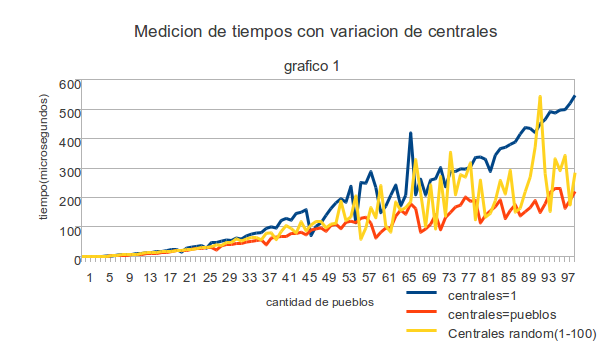
\includegraphics[width=0.8\textwidth]{grafico2-1.png}
  \label{fig:ejemplo}
\end{figure}

\paragraph{Gr�fico 2}
Para este gr�fico lo que hacemos es $constantizar$ el gr�fico 1, es decir, dividimos las mediciones 
por la complejidad que calculamos, en este caso $n^2$. \\

\begin{figure}[H]
    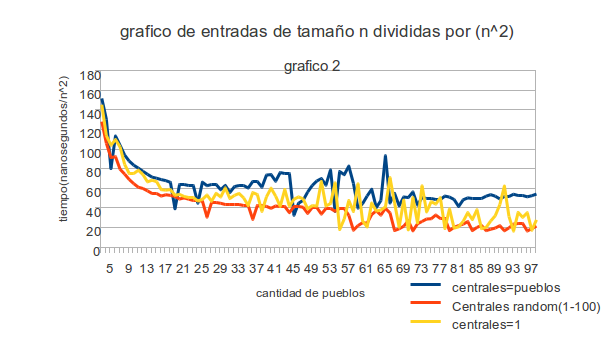
\includegraphics[width=0.8\textwidth]{grafico2-2.png}
  \label{fig:ejemplo}
\end{figure}

\subsubsection{Conclusiones} 
\paragraph{Gr�fico 1}
En este gr�fico se ven los dos casos extremos de C1:centrales = 1 y CN:centrales = numero de pueblos, se ve que claramente C1 es un peor caso y CN es un mejor caso, y que CR:centrales= (aleatorias entre 1 y el numero de pueblos)  oscila entre estos dos casos. esto muestra que la cantidad de centrales afecta al tiempo de computo del algoritmo, si bien esta acotada por el peor caso.

\paragraph{Gr�fico 2}
Queremos hacer notar que el gr�fico tiende a una constante, es decir, que efectivamente la complejidad es la esperada. para esto constantizamos los tres casos vistos en el grafico 1 para que se vea que la complejidad en peor y mejor caso queda constante al ser dividida por $n^2$ y que todos los otros casos oscilan entre estas dos constantes. \\

%\newpage

\section{Informe de modificaciones}

Solo se modific� el ejercicio tres. La modificaci�n es total.\\

\section{Problema 3: Saltos en \textit{la Matrix}}

\subsection{Descripci�n del Problema}

La \textit{Matrix} es un tablero de $n$ filas por $n$ columnas, por lo que contiene $n^2$ casilleros.
En cada casillero se encuentra un propulsor con una determinada potencia $p$, el cual puede usarse para moverse de manera vertical u horizontal $p$ 
casilleros. 

Adem�s cada jugador comienza con una cantidad $k$ de unidades de potencia extra que puede usar en cualquier salto, es decir, puede
 usar en un casillero de potencia $p'$ una cantidad $i$ de sus unidades de potencia extra para saltar $p'+i$ casilleros, pero esto implica que 
 le restan $k-i$ unidades de potencia extra para usar en el resto del juego. Si bien puede no usar todas sus unidades de potencia extra, 
 conservarlas no le reporta ning�n beneficio.
 
El juego comienza en un punto $X$, indicado como entrada del problema, perteneciente al tablero, y consiste en encontrar un camino que 
utilice la menor cantidad de saltos posibles para llegar a otro punto $Y$, tambi�n dado por entrada.


\subsubsection{Ejemplos}

Mostramos los siguientes ejemplos. Los detallamos en gr�ficos para mayor legibilidad. Los archivos usados para correr los tests se adjuntan con el c�digo. 

Las unidades de potencia de cada casillero aparecen detalladas en el gr�fico. La soluci�n, es decir, uno de los posibles caminos m�nimos 
en la cantidad de saltos, aparece como l�neas curvas entre casilleros. Las l�neas punteadas marcan a partir de qu� momento, en el salto, se usan unidades de potencia extra, si se usan.
Los c�rculos marcan los casilleros donde el jugador estuvo parado, es decir, donde empez� o termin� un salto. La casilla en amarillo marca el punto de inicio
de juego, y la casilla en naranja el punto de llegada. Las unidades de potencia extra se especifican debajo de cada gr�fico.

En ambos casos los caminos son soluciones pues no existen caminos entre los dos puntos que tengan menor cantidad de saltos.

\begin{figure}[H]
    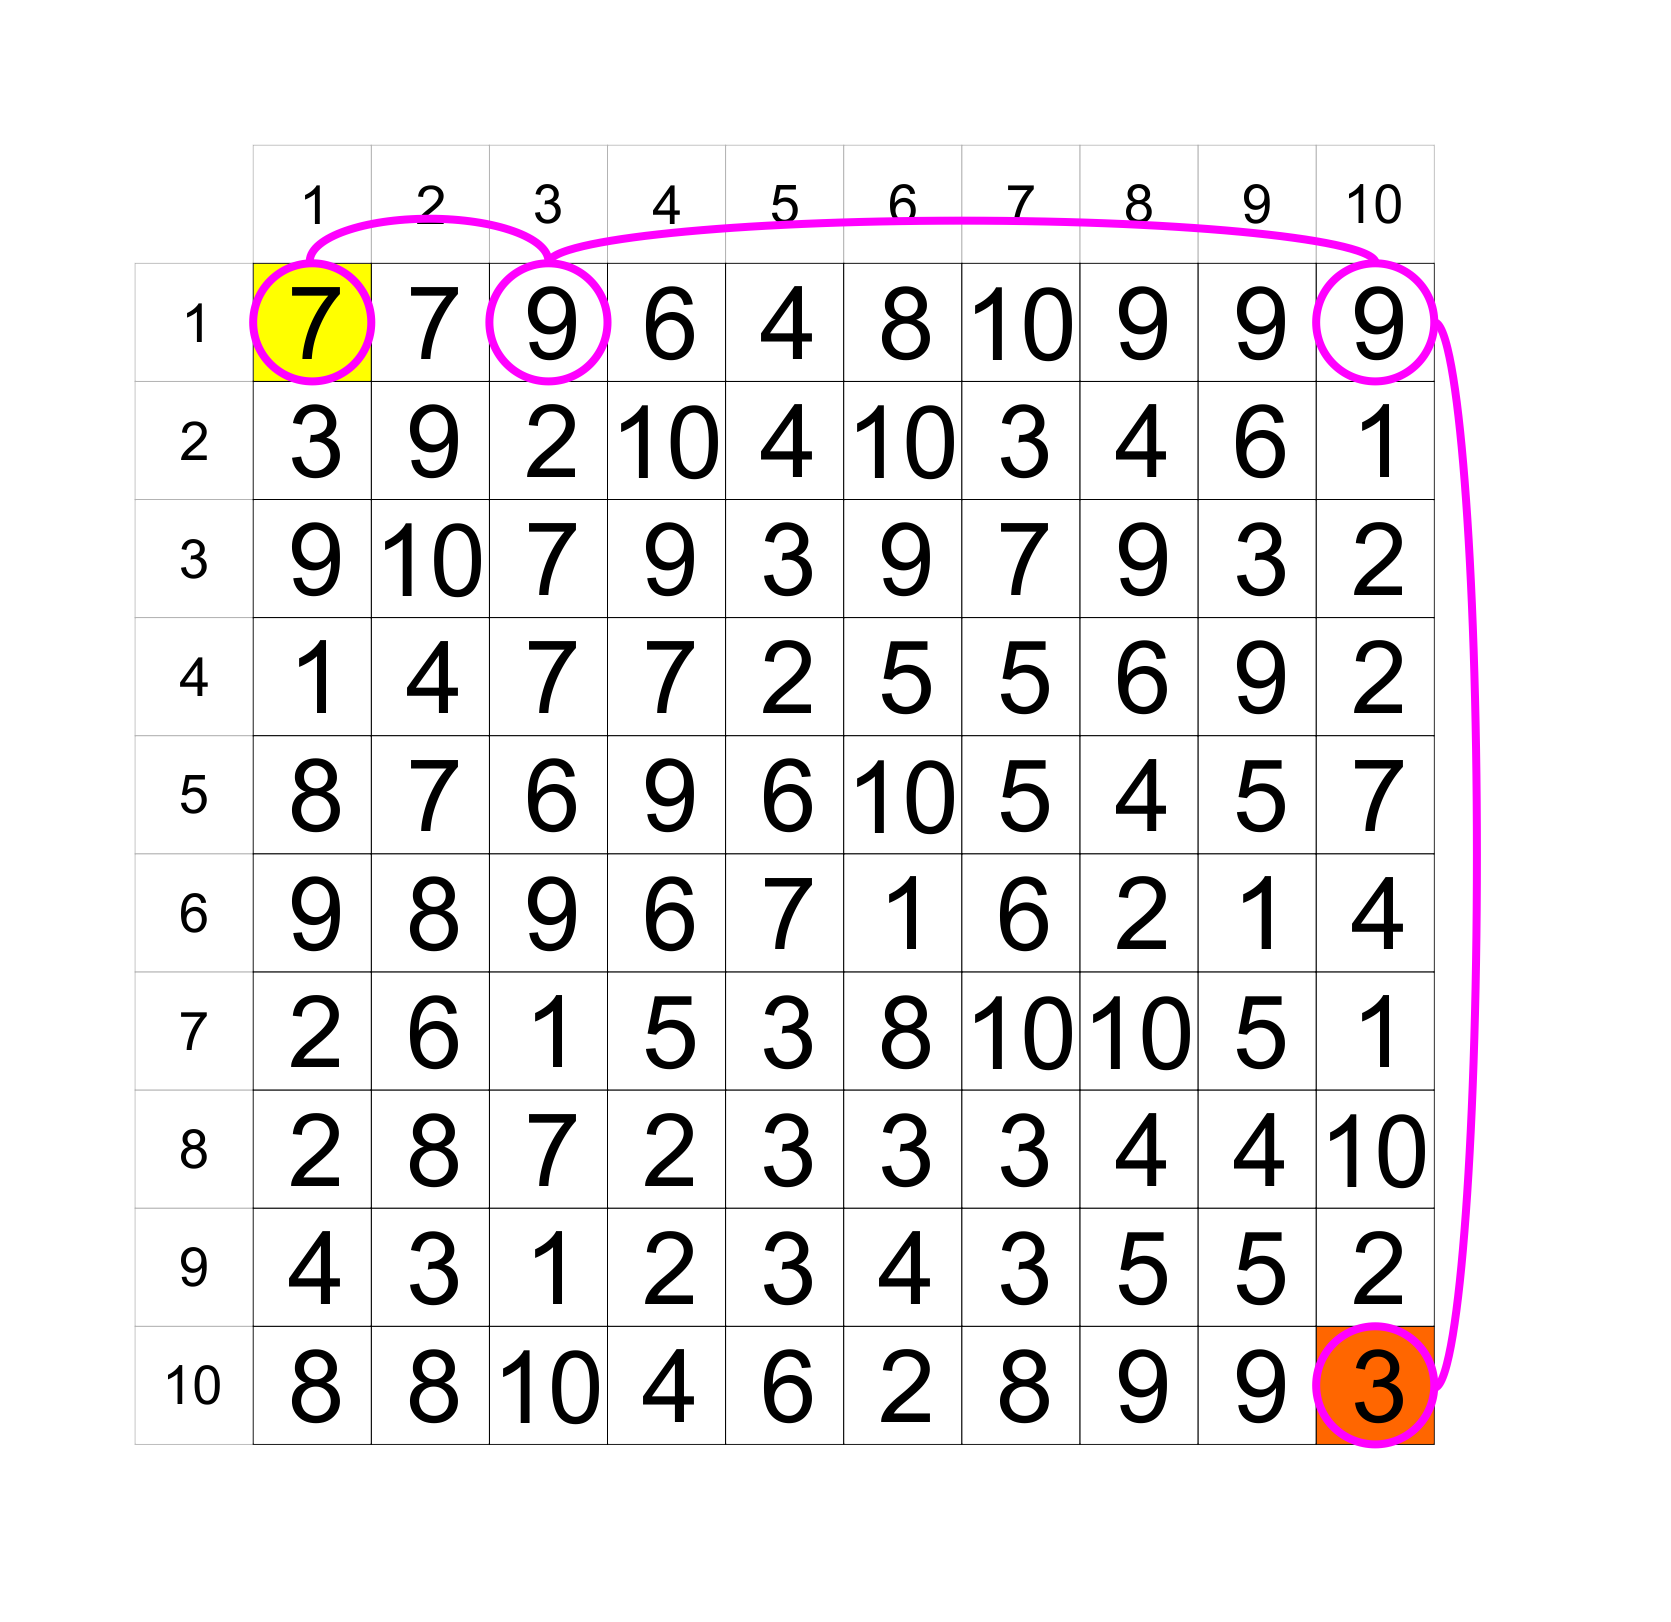
\includegraphics[width=0.4\textwidth]{epj1}
  \label{fig:ejemplo}
  \caption{Ejemplo con 0 unidades de potencia extra.}
\end{figure}

\begin{figure}[H]
    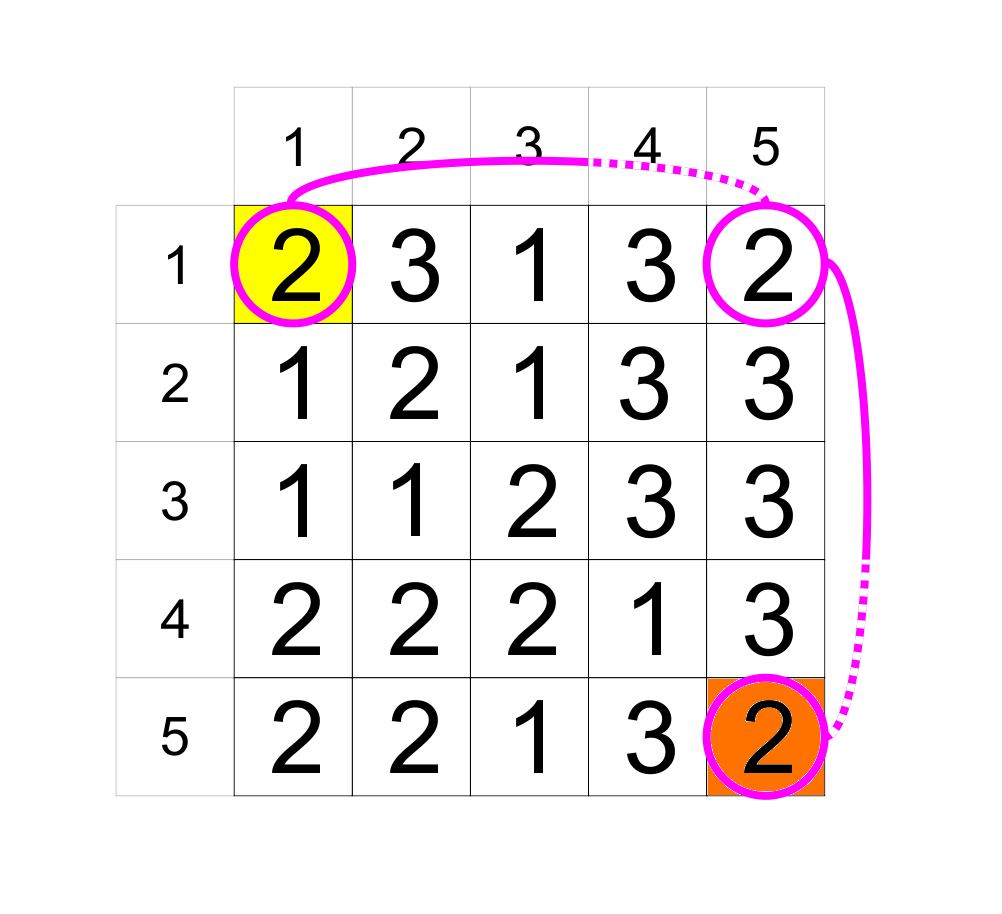
\includegraphics[width=0.3\textwidth]{epj2}
  \label{fig:ejemplo}
  \caption{Ejemplo con 4 unidades de potencia extra.}
\end{figure}

\paragraph{Nota:} La validez de estos casos se comprob� a mano.


\subsection{Resoluci�n}
Para resolver este problema, decidimos considerar al tablero y los saltos como un grafo con aristas dirigidas. En el grafo 
tomamos como v�rtices cada casillero del tablero y como aristas los posibles saltos de un casillero a otro. N�tese que las aristas son dirigidas,
pues que podamos ir de un casillero a otro no significa que podamos volver. Como lo que nos importa es la cantidad de saltos, todas las aristas 
tienen el mismo peso.

Gracias a que el peso de las aristas es siempre el mismo, podemos hacer BFS desde el casillero de inicio
y al encontrar el casillero de destino devolver el camino encontrado. De esta manera obtenemos uno de los caminos m�s cortos entre el
origen y el destino.


Luego extendemos este modelo para cuando tenemos potencia extra: lo que hacemos es tomar como v�rtices de este nuevo grafo $k+1$ 
conjuntos de nodos que se corresponden con un tablero cada uno. Lo que los diferencia es la cantidad de potencia extra disponible.
%Si el jugador se encuentra en el nodo de la posici�n $(1, 1)$ para la potencia extra $2$, entonces est� en esa posici�n y le quedan dos unidades de potencia extra. 
Necesitamos $k+1$ conjuntos para cubrir todos los valores posibles de potencia extra $k$, $k-1$, ..., 
$1$, $0$. Las aristas en este caso son los saltos posibles dentro de un nivel de potencia extra determinado, como en el caso anterior, y tambi�n
hacia un nivel de potencia extra 
inferior. N�tese que estas aristas que agregamos tambi�n son dirigidas pues nunca es posible ganar potencia extra haciendo un salto.
Como nuevamente las aristas representan saltos del jugador, sean potenciados o no, se puede usar BFS para encontrar el camino m�nimo hasta el 
destino.
% Por ejemplo si de la casilla v se puede llegar a la casilla $w$ usando 3 unidades de potencia extra, 
% entonces para cada $k > 4$ existir� el eje entre el v�rtice $v_k$ y $w_k-3$. Estas aristas que agregamos tambi�n son dirigidas, 
% pues nunca es posible ganar potencia extra haciendo un salto.  


\subsection{Correctitud}

Para demostrar correctitud tenemos que demostrar cuatro cosas:

\subsubsection{Definici�n 1: Una arista en G representa un salto en T}
Vamos a hablar de los nodos como una tupla (Casillero,PotenciaDisponible).
Por definici�n en el grafo G una arista $a$=<($o$,$k$),($d$,$k-i$)> representa que en el tablero se puede llegar desde un casillero origen $o$ hasta un casillero destino $d$, utilizando $i$ unidades de potencia extra, y siendo $k$ la potencia disponible antes de hacer el salto, con $i \leq k$. Por como se genera el grafo en nuestro algoritmo, si esa arista existe entonces representa un salto v�lido en T.

\subsubsection{Lema 1: Descartar saltos que derrochan energ�a extra es correcto, los saltos que no derrochan no se descartan}
Notamos que no consideramos como saltos v�lidos aquellos saltos donde las unidades de potencia extra se usen de manera in�til. 
A lo que nos referimos con 
esto es que si el jugador est� parado en un casillero P, con p unidades de potencia y le quedan k unidades de potencia extra, y salta a un 
casillero P' que est� a menos de p+1 casilleros de distancia, nuestro algoritmo no usa ninguna unidad de potencia extra. Del mismo modo, si salta
casillero P' que est� a p+i casilleros de distancia, el salto solo usa i unidades de potencia extra, y si i>k, el salto no es v�lido 
por el enunciado del problema en s�, por lo que ni siquiera consideramos estos casos. 
Aunque puede existir una soluci�n �ptima en la que se use unidades de potencia extra de esta forma, siempre existe una equivalente 
en la que no pasa. Es decir, si tenemos un
camino C entre dos nodos de k saltos, trivialmente podemos recorrer el mismo camino con k saltos sin usar unidades de potencia extra de
manera in�til.

\subsubsection{Lema 2: Un camino en T es representado en G si no derrocha energ�a} 


Sea C un camino entre el casillero de inicio (Xi,Yi) y un casillero cualquiera (X,Y), v�lido seg�n las reglas del 
juego y que no derrocha energ�a, queremos ver que 
C pertenece a G, donde G es el grafo que describimos en la resoluci�n. Para esto usaremos inducci�n en la longitud del camino.

CB1: camino trivial, sin saltos: Por definici�n, para cada potencia extra k, todo casillero de T esta representado 
en un v�rtice de G. asi que como existe el v�rtice en G entonces existe el camino.

CB2: camino de un salto: sean dos casilleros en T, $o$ y $d$ tal que existe un salto que va de $o$ a $d$. Por Lema 
1 ese salto esta representado en G, as� que existe una arista entre $o$ y $d$, por lo que existe un camino entre $o$ y $d$. 

HI: dado un camino $C$ de longitud n, o sea que realiza n saltos, v�lido seg�n las reglas del juego, $C$ pertenece a G.

Dado $C' = C'' ++ (i,j)$ donde $C'$ representa un camino en el tablero de $n+1$ saltos, construido por $C''$ un camino 
de $n$ saltos, $(i,j)$ el
�ltimo casillero del camino $C'$. Queremos ver que en G existe un camino que representa a $C'$.  


Por hip�tesis inductiva $C''$, un camino valido de n saltos (si no es valido entonces no existe en T), pertenece a G.
Adem�s sabemos que existe en T un salto entre el �ltimo nodo de $C''$, $(i',j')$, e $(i,j)$, pues si no existiese entonces C'
no seria un camino valido en T. Como es un camino v�lido, entonces existe este salto en T, luego, por el Lema 1,
existe en G una arista entre estos dos nodos. Luego, podemos formar $C'$ como la uni�n de estos caminos, entonces existe C' en G.

 
\subsubsection{Lema 3: Usamos BFS de manera correcta}

El c�digo implementado utiliza un BFS para encontrar el camino m�nimo entre el punto inicial y el
punto final. Esto es posible gracias a que las aristas no tienen pesos, as� que podemos suponer
que todos los pesos son iguales. Lo que hacemos es usar la funci�n ObtenerYMarcarPuntosAdyacentes
(OYMPA) para marcar todos los vecinos de un v�rtice como ya visitados y agregarlos a la lista de 
v�rtices a visitar, tambi�n para agregar a cada v�rtice su predecesor. Esto funciona exactamente 
igual que un BFS por lo que podemos encontrar el camino m�nimo en G y tambi�n reconstruirlo correctamente, 
usando los predecesores del punto final hasta llegar al punto de inicio y devolverlos. Por lema 4, el camino
devuelto por el BFS se corresponde con un camino m�nimo en T.

En la secci�n de complejidad se puede ver el pseudoc�digo de ObtenerYMarcarPuntosAdyacentes.

\subsubsection{Lema 4: Un camino m�nimo en G es un camino m�nimo en T}
Por el lema 2 sabemos que en G tenemos todos los caminos que no derrochan energ�a, y 
por el lema 1, sabemos que entre estos caminos siempre tenemos soluciones correctas en T. Como
las aristas representan la cantidad de saltos dados entonces encontrar el camino m�nimo en G 
es equivalente a encontrar un camino m�nimo en T.


\subsubsection{Conclusi�n}
Luego, por lema 3, conseguimos un camino m�nimo en G entre los dos puntos. Por lema 4,
sabemos que este camino se corresponde con un camino m�nimo en T.
Entonces el c�digo devuelve un camino m�nimo del juego Saltos en \textit{la Matrix}.







\newpage

\subsection{Complejidad}

Sea $n$ la cantidad de filas y columnas de la Matrix y $k$ la cantidad de unidades extra de potencia inicial.

\subsubsection{Funci�n principal}

\begin{algoritmo}{Resolver}{\In{laMatrix}{Matrix}, \In{potenciaExtra}{Nat}, \In{origen}{Coordenada}, \In{destino}{Coordenada}}[Lista(Par(Coordenada, Potencia))]
\LinesNumbered
\nl	LaTablita tabla(laMatrix.Filas(), potenciaExtra)\tcc*{$O$($n^2*k$)}
	\tcc{Rellenamos la tabla para el caso base.}
	tabla.Camino[origen.fila-1][origen.columna-1][potenciaExtra].Saltos \asignar 0\tcc*{$O$(1)}
	\tcc{Llenamos la tabla partiendo desde el punto de origen.}
	Lista(Par(Coordenada, Potencia)) puntosPorVer\tcc*{$O$(1)}
	ObtenerYMarcarPuntosAdyacentes(puntosPorVer, tabla, laMatrix, origen, potenciaExtra)\tcc*{$O$($n$)}
	\tcc{Este ciclo itera como mucho $k$ veces por cada casillero. Entonces itera $n^2*k$ veces en el peor caso.}
	\While(\tcc*[f]{$O$(1)}){$\neg$puntosPorVer.Vacia()}{
		Coordenada pos \asignar puntosPorVer.Primero().coordenada\tcc*{$O$(1)}
		Nat potenciaDisponible \asignar puntosPorVer.Primero().potencia\tcc*{$O$(1)}
		puntosPorVer.BorrarPrimero()\tcc*{$O$(1)}
		ObtenerYMarcarPuntosAdyacentes(puntosPorVer, tabla, laMatrix, pos, potenciaDisponible)\tcc*{$O$($n^2*k*n$)}
	}
	res \asignar tabla.CaminoMinimo(destino)\tcc*{$O$($n+k$)}

\end{algoritmo}

El constructor de la tabla inicializa todas las posiciones colocando el atributo Saltos en $-1$ para indicar que est� indefinido. Como tiene tama�o $n^2*(k+1)$, el costo de inicializarlo es $O$($n^2*k$).

Como se ejecuta ObtenerYMarcarPuntosAdyacentes cuya complejidad es $O$($n$) dentro del ciclo que itera en el orden de $n^2*k$ veces, la complejidad es de $O$($n^3*k$) para el ciclo. El resto de las operaciones tienen un costo que est� incluido en $O$($n^3*k$). M�s adelante vemos por qu� itera no m�s de $n^2*k$ veces el ciclo.


\subsubsection{Funci�n an�loga a BFS}

\begin{algoritmo}{ObtenerYMarcarPuntosAdyacentes}{\Inout{puntosPorVer}{Lista(Par(Coordenada, Potencia))}, \Inout{tabla}{LaTablita}, \In{laMatrix}{Matrix}, \In{pos}{Coordenada}, \In{destinoAbsoluto}{Coordenada}, \In{potenciaDisponible}{Nat}}
\LinesNumbered
\nl	
	Int potencia \asignar laMatrix.PotenciaDe(pos)\tcc*{$O$(1)}
	\tcc{Itera $O$($n$) veces.}
	\For(\tcc*[f]{$O$(1)}){\Forcond{i \asignar -potencia}{potencia}}{
		Coordenada posDestino \asignar <pos.Fila+i, pos.Columna>\tcc*{$O$(1)}
		MarcarYAgregar(puntosPorVer, pos, posDestino, tabla, potenciaDisponible, 0)\tcc*{$O$(1)}
		Si marqu� el destino absoluto, limpio la lista de puntos por ver y retorno a la funci�n que me llam�.\tcc*{$O$(1)}
		posDestino.Fila \asignar pos.Fila\tcc*{$O$(1)}
		posDestino.Columna \asignar posDestino.Columna + i\tcc*{$O$(1)}
		MarcarYAgregar(puntosPorVer, pos, posDestino, tabla, potenciaDisponible, 0)\tcc*{$O$(1)}
		Si marqu� el destino absoluto, limpio la lista de puntos por ver y retorno a la funci�n que me llam�.\tcc*{$O$(1)}
	}
	
	\tcc{Itera $O$($k$) veces.}
	\For(){\Forcond{potenciaExtra \asignar 1}{potenciaDisponible}} {
		Nat potenciaTotal \asignar potencia + potenciaExtra\tcc*{$O$(1)}
		Coordenada posDestino \asignar <pos.Fila-potenciaTotal, pos.Columna>\tcc*{$O$(1)}
		MarcarYAgregar(puntosPorVer, pos, posDestino, tabla, potenciaDisponible, potenciaExtra)\tcc*{$O$(1)}
		Si marqu� el destino absoluto, limpio la lista de puntos por ver y retorno a la funci�n que me llam�.\tcc*{$O$(1)}
		
		posDestino.Fila \asignar posDestino.Fila + 2*potenciaTotal\tcc*{$O$(1)}
		MarcarYAgregar(puntosPorVer, pos, posDestino, tabla, potenciaDisponible, potenciaExtra)\tcc*{$O$(1)}
		Si marqu� el destino absoluto, limpio la lista de puntos por ver y retorno a la funci�n que me llam�.\tcc*{$O$(1)}
		
		posDestino.Fila \asignar pos.Fila\tcc*{$O$(1)}
		posDestino.Columna \asignar posDestino.Columna - potenciaTotal\tcc*{$O$(1)}
		MarcarYAgregar(puntosPorVer, pos, posDestino, tabla, potenciaDisponible, potenciaExtra)\tcc*{$O$(1)}
		Si marqu� el destino absoluto, limpio la lista de puntos por ver y retorno a la funci�n que me llam�.\tcc*{$O$(1)}
		
		posDestino.Columna \asignar posDestino.Columna + 2*potenciaTotal\tcc*{$O$(1)}
		MarcarYAgregar(puntosPorVer, pos, posDestino, tabla, potenciaDisponible, potenciaExtra)\tcc*{$O$(1)}
		Si marqu� el destino absoluto, limpio la lista de puntos por ver y retorno a la funci�n que me llam�.\tcc*{$O$(1)}
	}
\end{algoritmo}

Limpiar la lista puntosPorVer puede costar $O$($n^2*k$) en el peor caso pero hacerlo implica la terminaci�n del ciclo de la funci�n principal, con lo cual no afecta su complejidad. Por razones que explicaremos m�s adelante esta funci�n tiene costo $O$($n$) en el peor caso.


\subsubsection{Funci�n de marcado de v�rtices}

\begin{algoritmo}{MarcarYAgregar}{\Inout{puntosPorVer}{Lista(Par(Coordenada, Potencia))}, \In{pos}{Coordenada}, \In{posDestino}{Coordenada}, \Inout{tabla}{LaTablita}, \In{potenciaDisponible}{Nat}, \In{potenciaExtra}{Nat}}
\LinesNumbered
\nl	
	\If(\tcc*[f]{$O$(1)}) {$\neg$laMatrix.EsCoordenadaValida(posDestino)} {
		\return\tcc*{$O$(1)}
	}
	CaminoMin origen \asignar tabla.distancia[posOrigen.Fila-1][posOrigen.Columna-1][potenciaDisponible]\tcc*{$O$(1)}
	CaminoMin destino \asignar tabla.distancia[posDestino.Fila-1][posDestino.Columna-1][potenciaDisponible-potenciaExtra]\tcc*{$O$(1)}
	\If(\tcc*[f]{$O$(1)}) {destino.Saltos == -1}{
		lista.AgregarAtras(<posDestino, potenciaDisponible-potenciaExtra>)\tcc*{$O$(1)}
	}
	\If(\tcc*[f]{$O$(1)}) {destino.Saltos == -1 $\lor$ destino.Saltos > origen.Saltos+1} {
		destino.Saltos = origen.Saltos+1\tcc*{$O$(1)}
		destino.CasilleroAnterior = posOrigen\tcc*{$O$(1)}
		destino.potenciaUsada = potenciaExtra\tcc*{$O$(1)}
	}
\end{algoritmo}

En MarcarYAgregar se retorna de inmediato si la coordenada para marcar es inv�lida. Por esto, se puede acotar el costo del segundo ciclo de ObtenerYMarcarPuntosAdyacentes al costo de las, como mucho, $2n-2$ llamadas que tienen coordenadas v�lidas. 
Esto es porque en el peor caso la potencia del casillero es $1$ lo que implica que el ciclo abarca todos los saltos del origen a los casilleros en la misma fila y todos los saltos del origen a los casilleros en la misma columna quitando los dos que son adyacentes al estar en una esquina del tablero. 
Si no estuviera en una esquina del tablero, tendr�a tres o cuatro casilleros adyacentes que nunca mirar�a, reduciendo el costo total del ciclo. Entonces el costo del ciclo en peor caso es $O$($min(n, k)$). Finalmente esto hace que la complejidad de ObtenerYMarcarPuntosAdyacentes sea del orden $O$($n+min(n, k)$) que est� incluido en $O$($n$).

Se puede ver adem�s en el pseudoc�digo de MarcarYAgregar que si un nodo ya fue marcado (Saltos no vale $-1$) no se agrega a la lista de puntos por ver. Esto implica que la funci�n principal nunca puede recorrer m�s que la cantidad total de nodos del grafo. La cual es $n^2*k$. Por lo tanto itera, esa cantidad de veces en el peor caso.

\subsubsection{Funci�n de reconstrucci�n del camino}

\begin{algoritmo}{CaminoMinimo}{\In{tabla}{LaTablita}, \In{pos}{Coordenada}}[Lista(Par(Coordenada, Potencia))] {
	CaminoMin este\tcc*{$O$(1)}
	Nat potenciaFinal \asignar 0\tcc*{$O$(1)}
	\tcc{Itera $k+1$ veces en el peor caso.}
	\For(\tcc*[f]{$O$(1)}) {\Forcond{k \asignar 0}{tabla.potenciaMaxima}} {
		vector<CaminoMin> caminos \asignar tabla.distancia[pos.first-1][pos.second-1]\tcc*{$O$(1)}
		\If(\tcc*[f]{$O$(1)}) {caminos[k].Saltos $\neq$ -1} {
			este \asignar caminos[k]\tcc*{$O$(1)}
			potenciaFinal \asignar k\tcc*{$O$(1)}
			\Break\tcc*{$O$(1)}
		}
	}
	CoordenadaYPotencia paso\tcc*{$O$(1)}
	paso.Posicion \asignar pos\tcc*{$O$(1)}
	paso.Potencia \asignar este.potenciaUsada\tcc*{$O$(1)}
	\tcc{Itera $2n$ veces en el peor caso.}
	\While(\tcc*[f]{$O$(1)}) {este.Saltos > 0} {
		res.AgregarAdelante(paso)\tcc*{$O$(1)}
		potenciaFinal \asignar potenciaFinal + este.potenciaUsada\tcc*{$O$(1)}
		Coordenada anterior \asignar este.CasilleroAnterior\tcc*{$O$(1)}
		este \asignar tabla.distancia[anterior.first-1][anterior.second-1][potenciaFinal]\tcc*{$O$(1)}
		paso.Posicion \asignar anterior\tcc*{$O$(1)}
		paso.Potencia \asignar este.potenciaUsada\tcc*{$O$(1)}
	}
}
\end{algoritmo}
Vale aclarar que el segundo ciclo no puede iterar m�s de $2n$ veces porque no existe un camino m�nimo entre el origen y el destino que puedan tomar m�s de $2n$ saltos siendo $n$ la cantidad de filas y columnas de la matrix. Esto es porque todo casillero tiene por lo menos una unidad de potencia en el resorte.
Sumando los �rdenes de complejidad de peor caso para ambos ciclos da $O$($n+k$). Como esto est� incluido en $O$($n*k$), no afecta a la complejidad de la funci�n principal.


\subsubsection{Conclusi�n}

La complejidad de peor caso del algoritmo implementado es $O$($n^3*k$) por lo anteriormente expuesto.



\subsection{Testing}

Para testear correctitud usamos los siguientes ejemplos. Los detallamos en gr�ficos para mayor legibilidad. Los archivos usados para correr los tests se adjuntan con el c�digo.

Las unidades de potencia de cada casillero aparecen detalladas en el gr�fico. La soluci�n, es decir, uno de los posibles caminos m�nimos 
en la cantidad de saltos, aparece como l�neas curvas entre casilleros. Las l�neas punteadas marcan a partir de qu� momento, en el salto, se usan unidades de potencia extra, si se usan.
Los c�rculos marcan los casilleros donde el jugador estuvo parado, es decir, donde empez� o termin� un salto. La casilla en amarillo marca el punto de inicio
de juego, y la casilla en naranja el punto de llegada. Las unidades de potencia extra se especifican debajo de cada gr�fico.

En todos los casos la correctitud de las soluciones fue corroborada a mano.

\subsubsection{Test: No salta en diagonal}
\begin{figure}[H]
    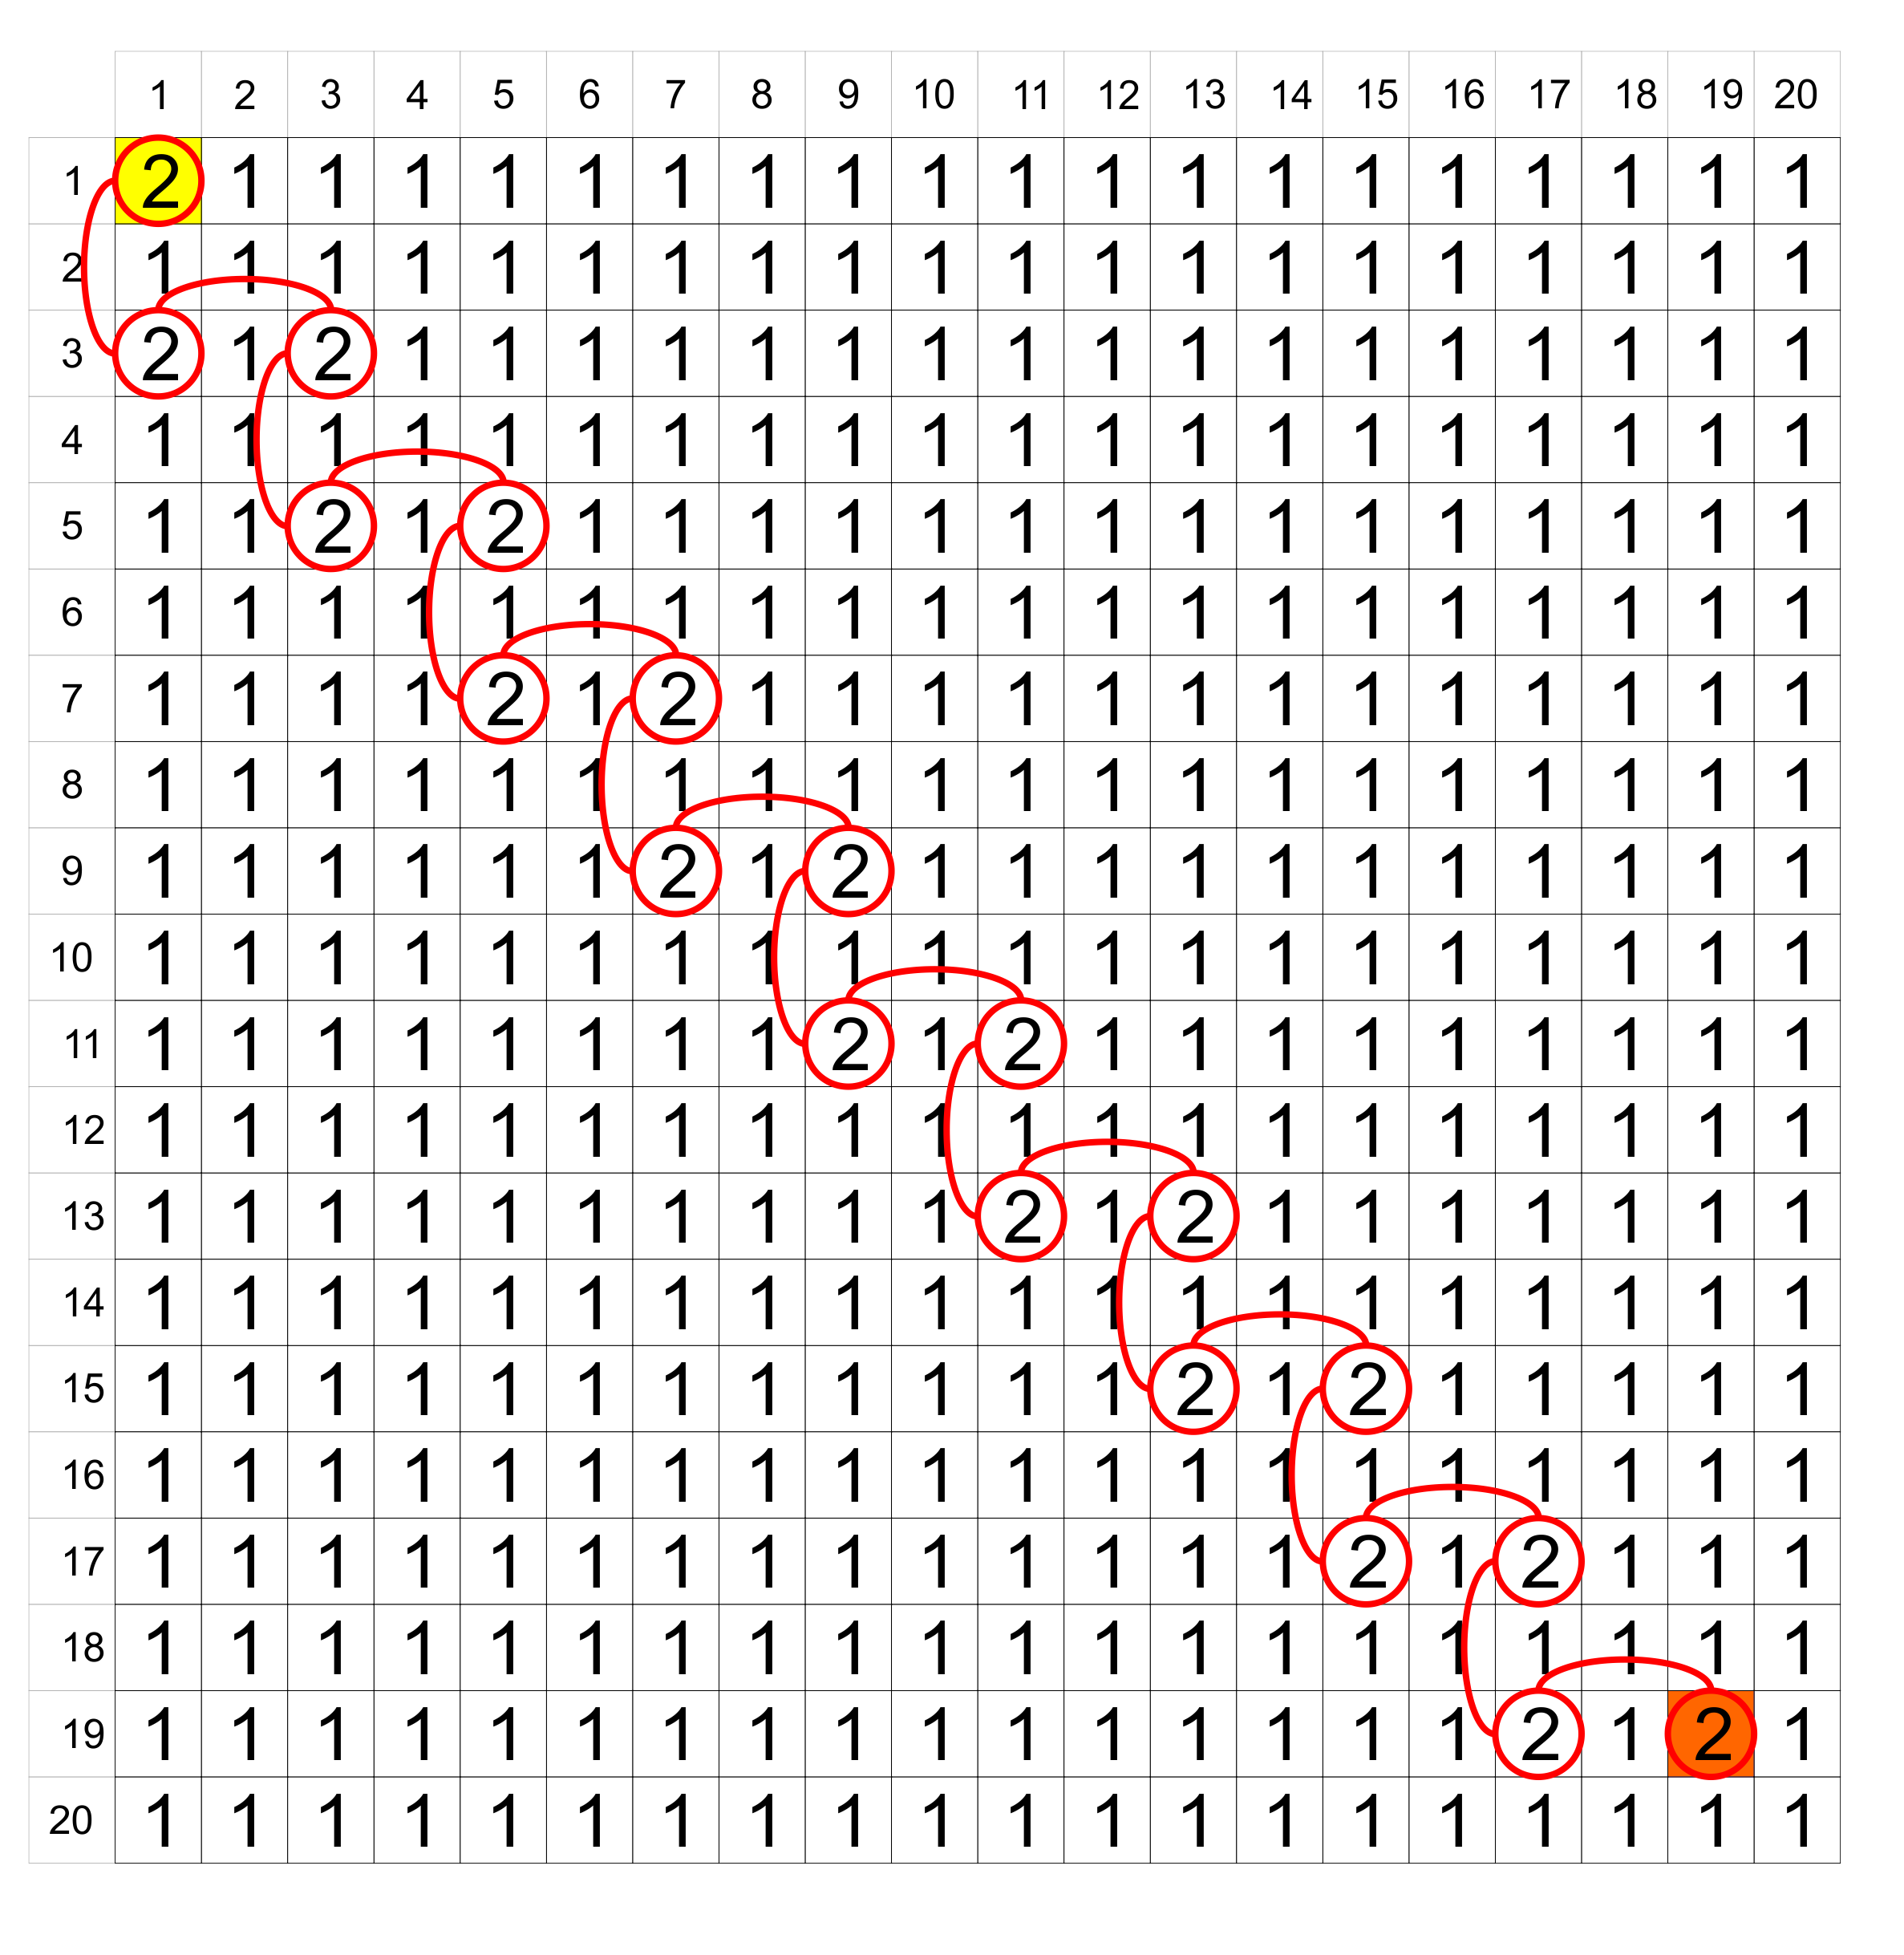
\includegraphics[width=0.8\textwidth]{ept1}
  \label{fig:ejemplo}
  \caption{Test con 0 unidades de potencia extra.}
\end{figure}

\subsubsection{Test: Tiene sentido com�n}
Lo que queremos comprobar con este test es que el algoritmo no usa \textit{golosamente} las unidades de potencia extra, sino que las usa apropiadamente para minimizar la cantidad de saltos.
\begin{figure}[H]
    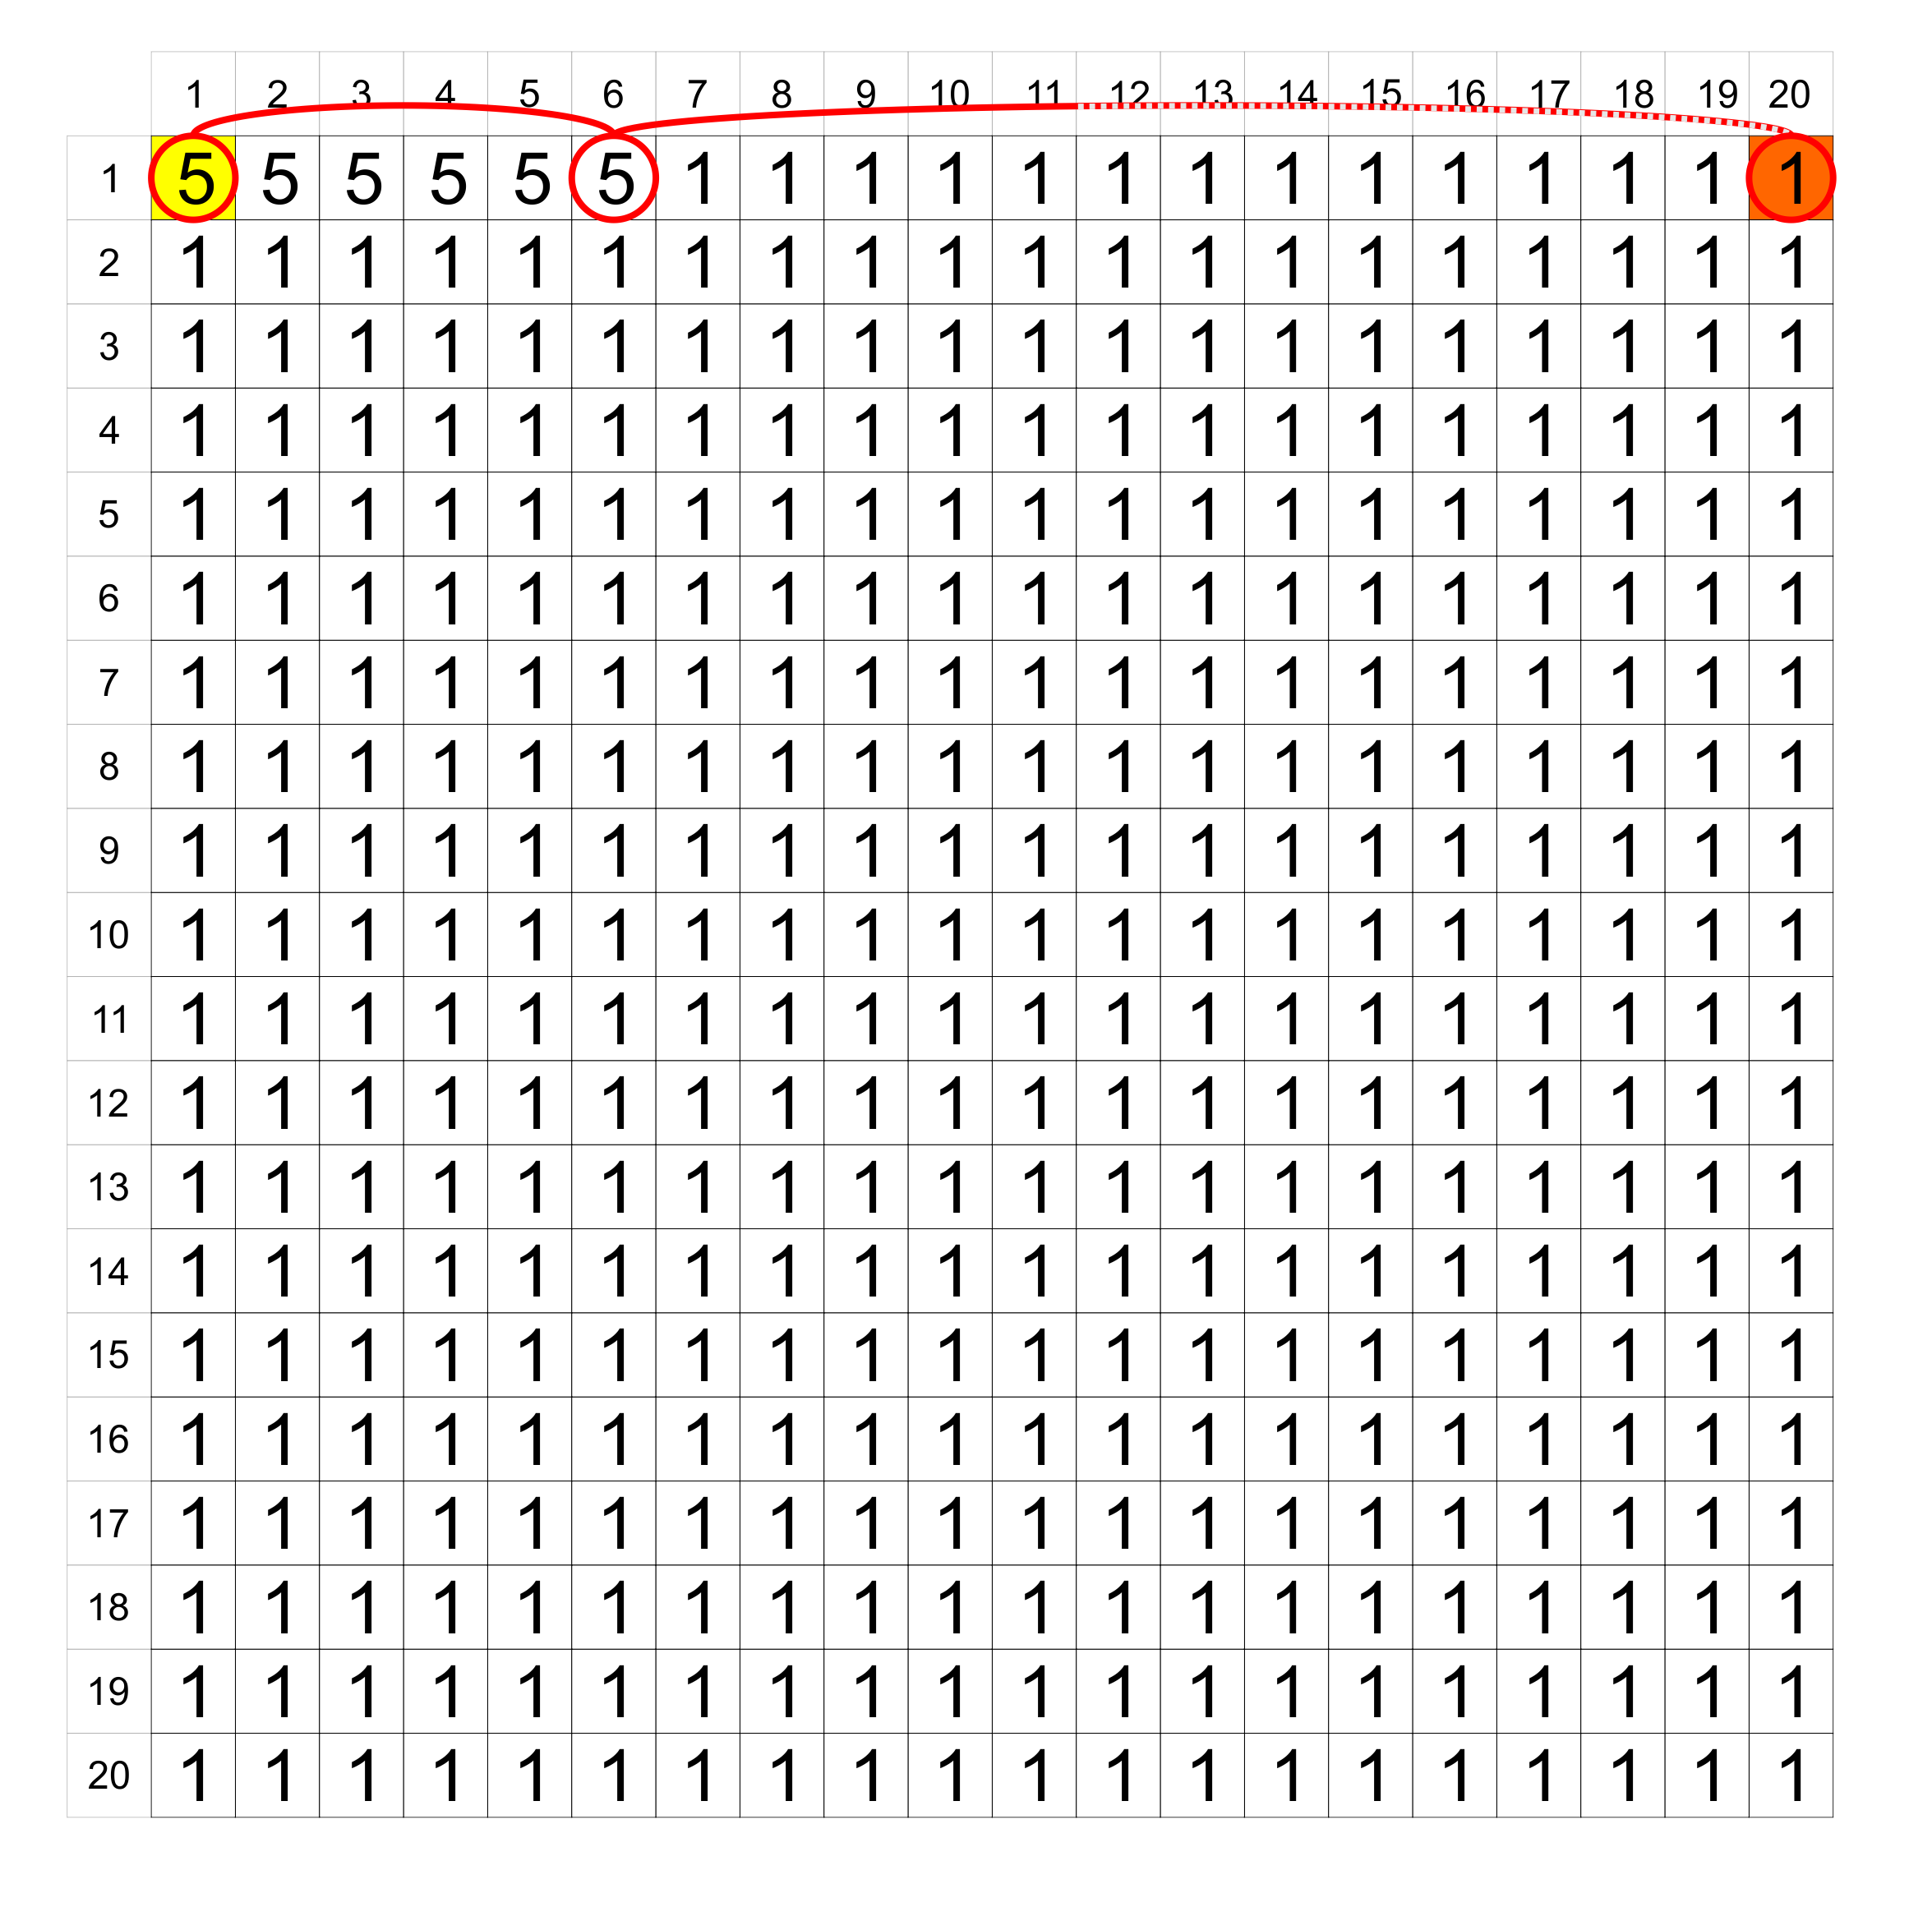
\includegraphics[width=0.8\textwidth]{ept2}
  \label{fig:ejemplo}
  \caption{Test con 10 unidades de potencia extra.}
\end{figure}

\subsubsection{Test: Caso borde}
Queremos comprobar que el algoritmo puede devolver una soluci�n �ptima si todos los elementos son iguales.
\begin{figure}[H]
    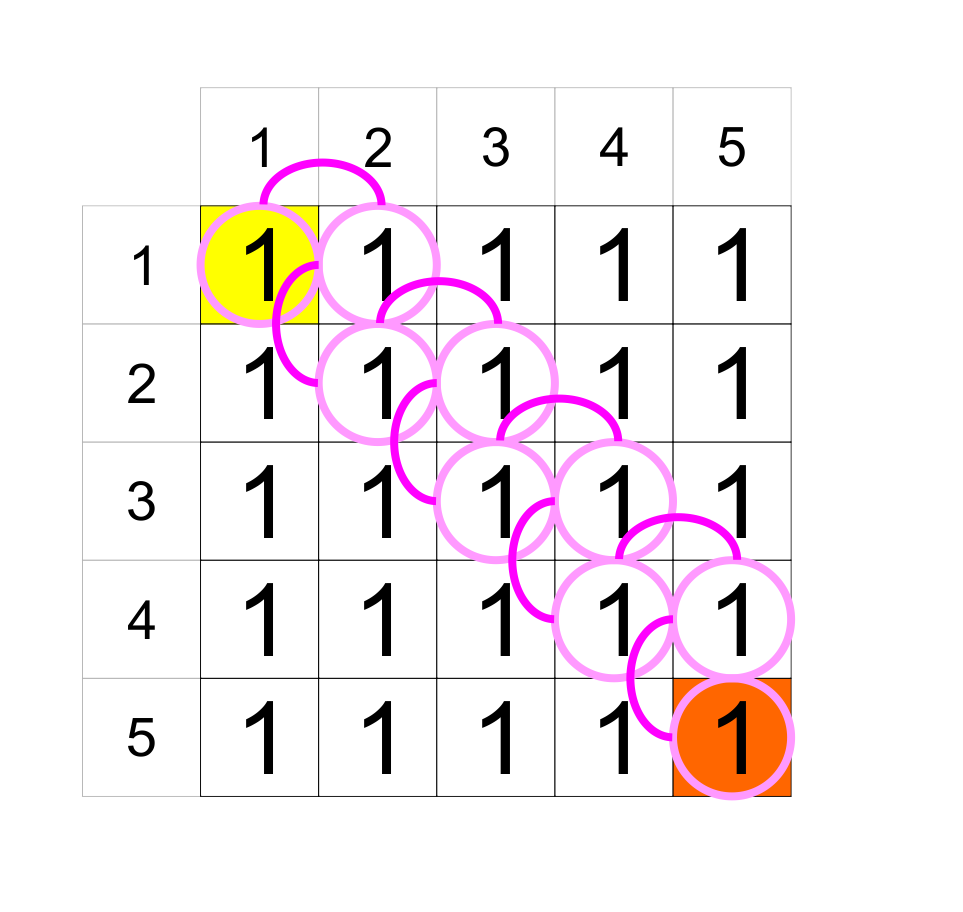
\includegraphics[width=0.3\textwidth]{ept3}
  \label{fig:ejemplo}
  \caption{Test con 0 unidades de potencia extra.}
\end{figure}

\subsubsection{Test: Retrocede si es la mejor elecci�n}
\begin{figure}[H]
    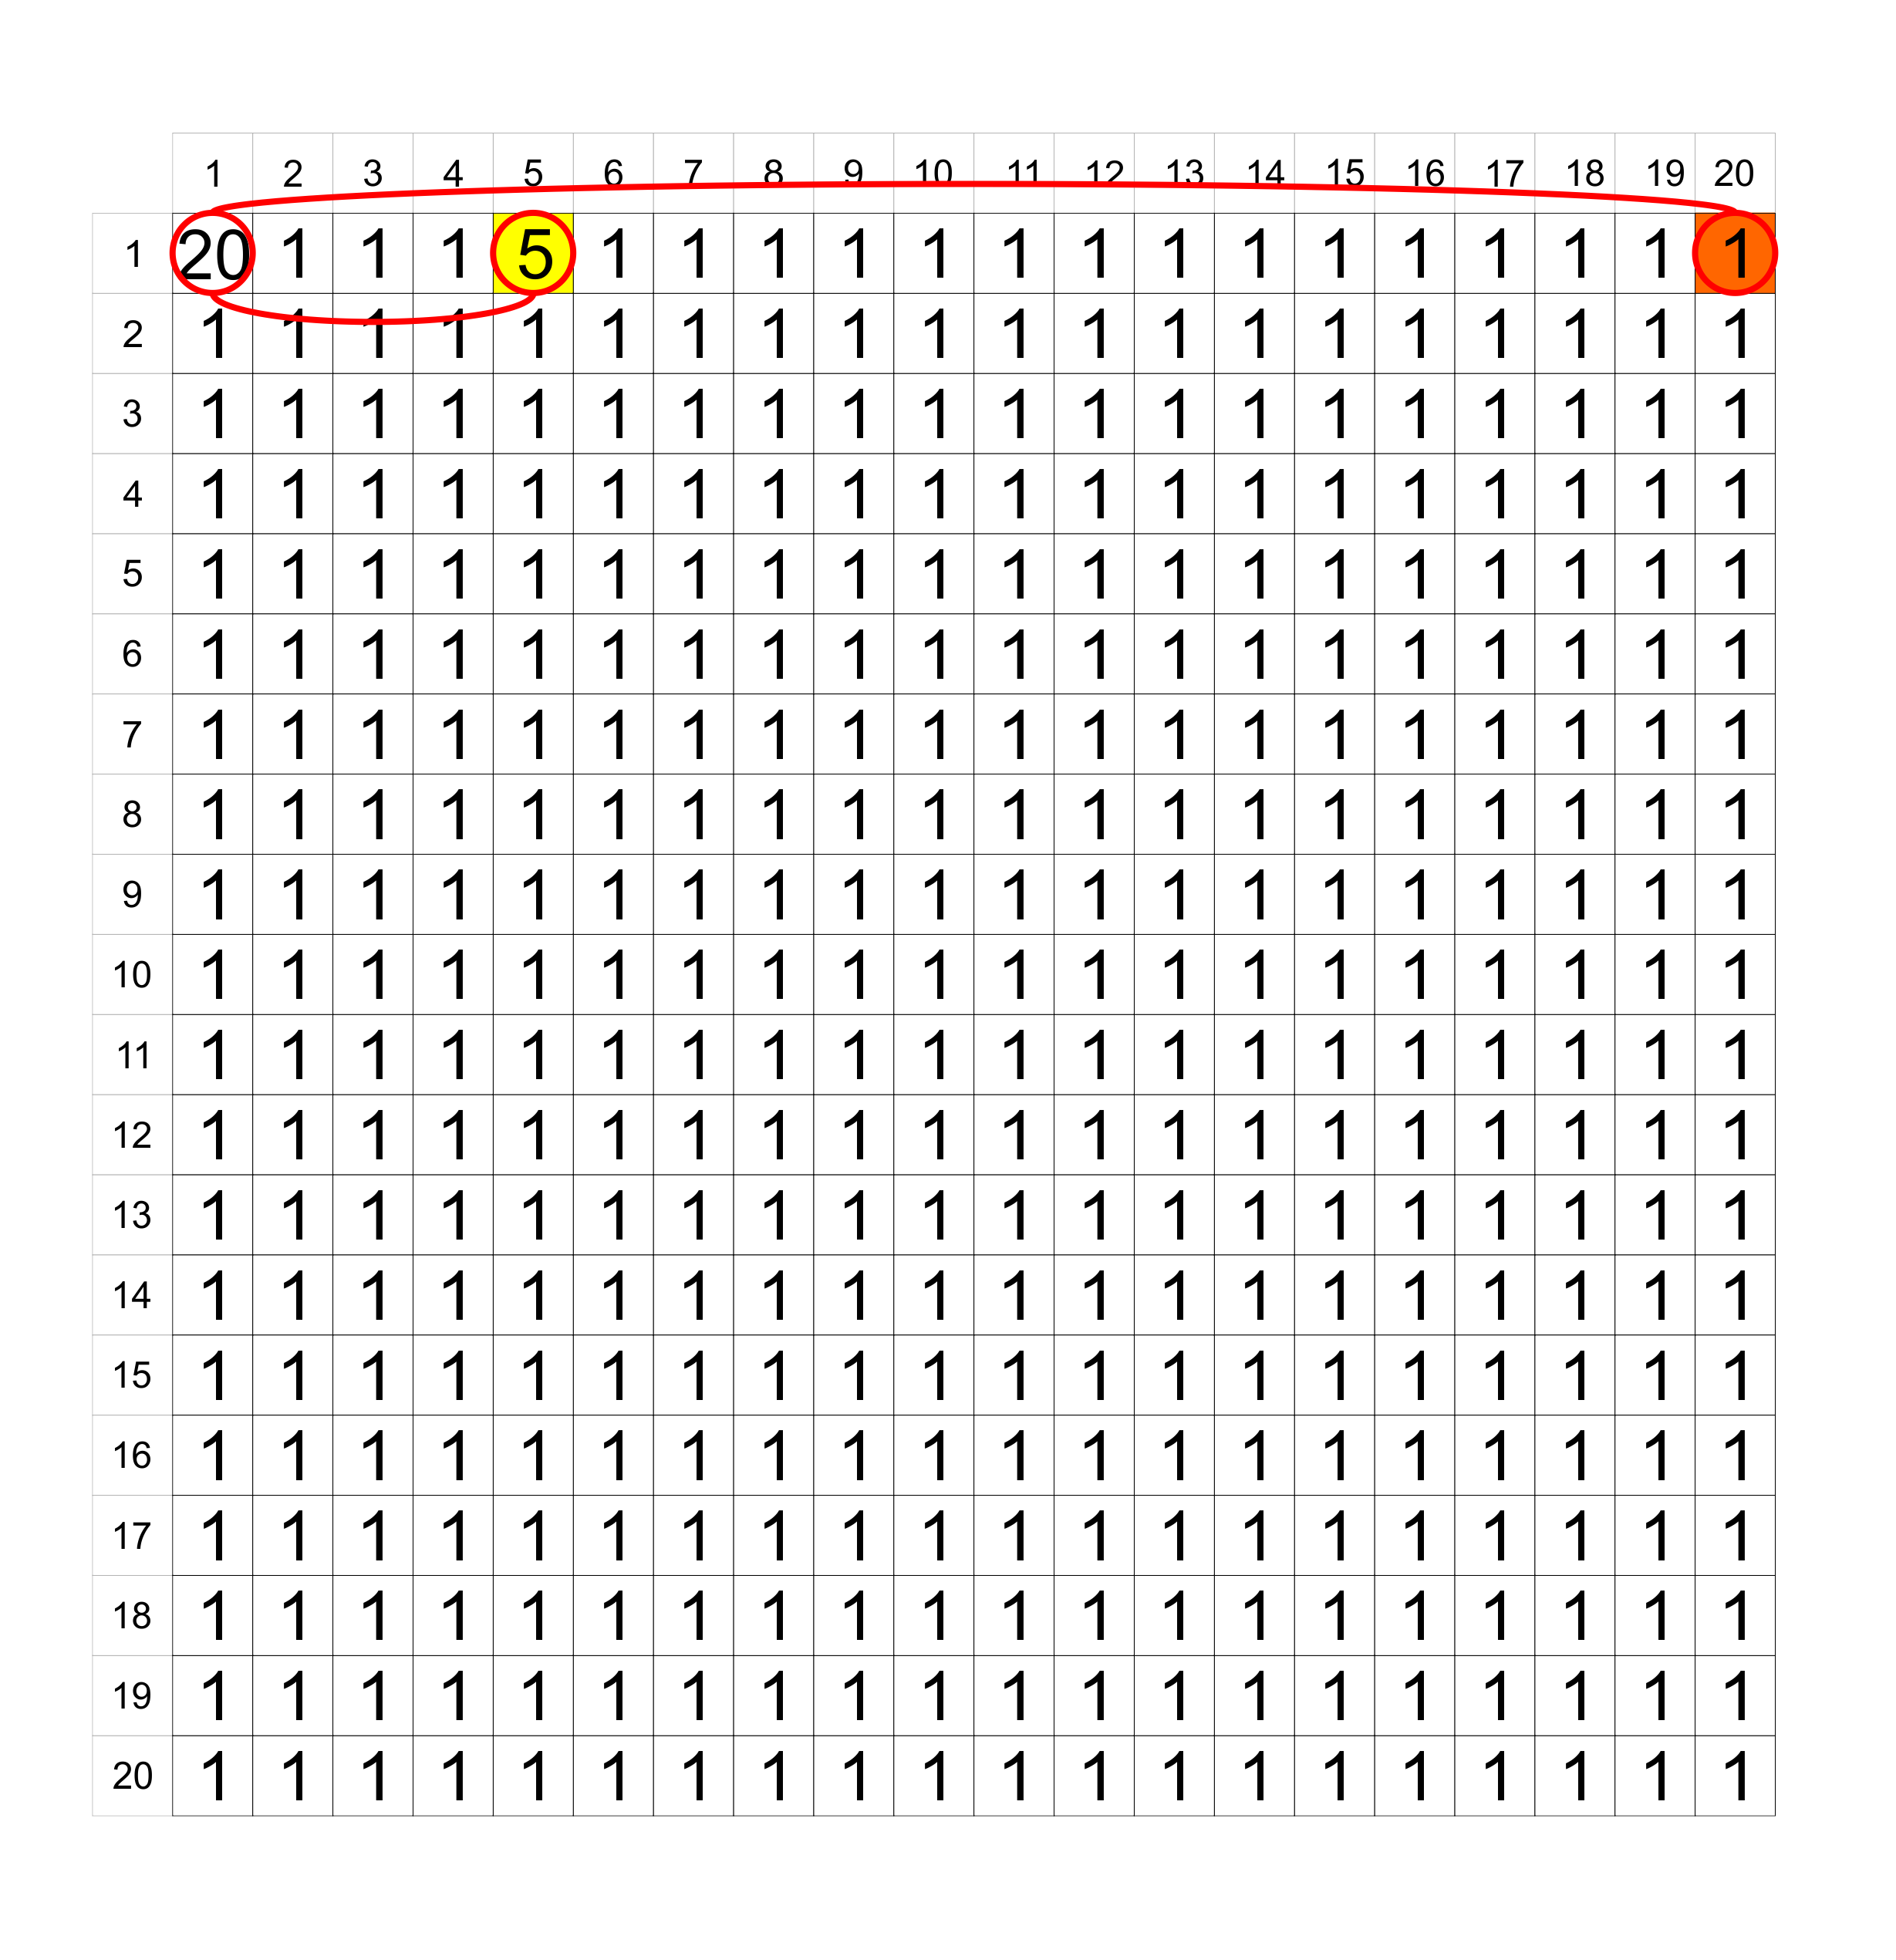
\includegraphics[width=0.8\textwidth]{ept4}
  \label{fig:ejemplo}
  \caption{Test con 0 unidades de potencia extra.}
\end{figure}

\subsubsection{Test: Caso borde}
Queremos comprobar que el algoritmo puede devolver una soluci�n �ptima si no tiene que hacer nada.
\begin{figure}[H]
    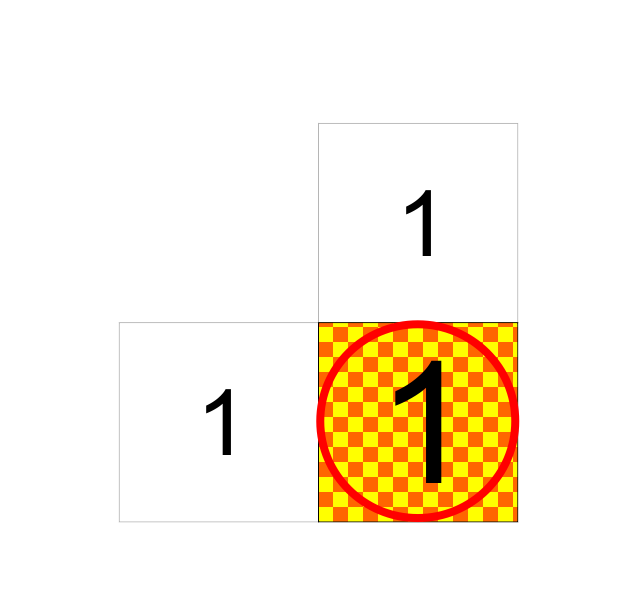
\includegraphics[width=0.1\textwidth]{ept5}
  \label{fig:ejemplo}
  \caption{Test con 0 unidades de potencia extra.}
\end{figure}

\subsection{Experimentaci�n}

En la experimentaci�n utilizamos dos generadores de instancias distintos. Uno utiliza valores pseudoaleatorios para rellenar los valores de potencia de los casilleros, la potencia extra y las coordenadas de partida y llegada. Todos los valores de potencia est�n acotados por los par�metros de entrada del generador.

El otro es un generador de valores constantes. Fija como punto de partida la esquina superior izquierda (cuya coordenada es ($1$,$1$)) y de llegada, la esquina inferior derecha (cuya coordenada es ($n$,$n$)). Adem�s utiliza los par�metros de entrada para definir la de todos los casilleros y la potencia extra de la instancia, en lugar de usarlo como cota superior.

Ambos generadores utilizan un �nico valor de $n$ para las instancias generadas. Esto significa que en un archivo tenemos las instancias para un cierto valor de $n$. Para medir el tiempo de ejecuci�n utilizamos un script de shell de linux que ejecuta una instancia del programa con cada archivo generado. Vale notar entonces que el programa termina completamente al finalizar con las instancias de cierto valor de $n$.

\subsubsection{Instancias aleatorias}
Utilizando un script de shell de linux, generamos $100$ instancias para cada valor de $n$ m�ltiplo de $10$ entre $10$ y $350$. El script usado en este caso fue \textbf{generar\_tests.sh}. Para generar instancias aleatorias utiliz� el generador pseudoaleatorio descripto anteriormente. Este script toma dos par�metros de entrada y opcionalmente un tercer par�metro. Los primeros dos definen el $n$ m�s chico y el m�s grande respectivamente para el cual generar instancias. El par�metro opcional determina el incremento con el cual se recorre el conjunto de n�meros entre el m�nimo y m�ximo. Para esta serie de instancias utilizamos el valor por defecto, $10$.

Adem�s internamente define la cota de potencia de los casilleros y la potencia extra como un cociente entre $n$ y un valor constante. Decidimos que este valor sea $3$. La idea de acotar la potencia es evitar la abundancia de tableros donde hay tanta potencia en los casilleros y en las reservas del jugador que existe un camino de uno o dos saltos al destino sea cual sea el origen. Al ser la cota $n/3$ s�lo van a existir tableros que se resuelven en uno o dos saltos si el destino ya se encontraba lo suficientemente cerca del origen.

\subsubsection{Instancias Dif�ciles}
Utilizando un script similar al anterior, generamos $100$ instancias para cada valor de $n$ m�ltiplo de $10$ entre $10$ y $350$. Sin embargo por el gran costo computacional s�lo pudimos resolver y medir instancias de este tipo hasta $n=180$. El script en este caso utiliz� el generador de valores constantes. Cabe destacar que las cien instancias generadas son todas id�nticas para cada valor de $n$ distinto.

El valor de potencia para estas instancias fue $n/3$. Esto significa que el jugador dispone de $n/3$ unidades de potencia extra y todo casillero tiene $n/3$ unidades de potencia para su resorte. La idea de usar el mismo valor que la cota de la serie aleatoria es poder comparar y ver cu�n dif�ciles son estas instancias contra las generadas aleatoriamente.

\subsubsection{Instancias F�ciles sin potencia extra}
Utilizando un script similar a los anteriores, generamos $100$ instancias para cada valor de $n$ m�ltiplo de $10$ entre $10$ y $350$. Nuevamente usamos el generador de valores constantes. En este caso la potencia de los casilleros es $n$ y la potencia extra, $0$. La idea de esta serie es comparar la dificultad de estas instancias con las aleatorias.

\subsubsection{Instancias F�ciles con potencia extra}
Utilizando un script similar a los anteriores, generamos $100$ instancias para cada valor de $n$ m�ltiplo de $10$ entre $10$ y $350$. Nuevamente usamos el generador de valores constantes. En este caso la potencia de los casilleros es $1$ y la potencia extra, $2n$. La idea de esta serie es comparar la dificultad de estas instancias con las aleatorias.

\subsubsection{Gr�ficos}

Como s�lo pudimos medir tests dif�ciles hasta $n=180$, filtramos las mediciones de los tests aleatorios hasta ese $n$ tambi�n. Los tests f�ciles con potencia extra sufrieron un corte similar, en lugar de $n=180$, los cortamos en $n=130$ porque el factor $k$ es $2n$ en ellos.

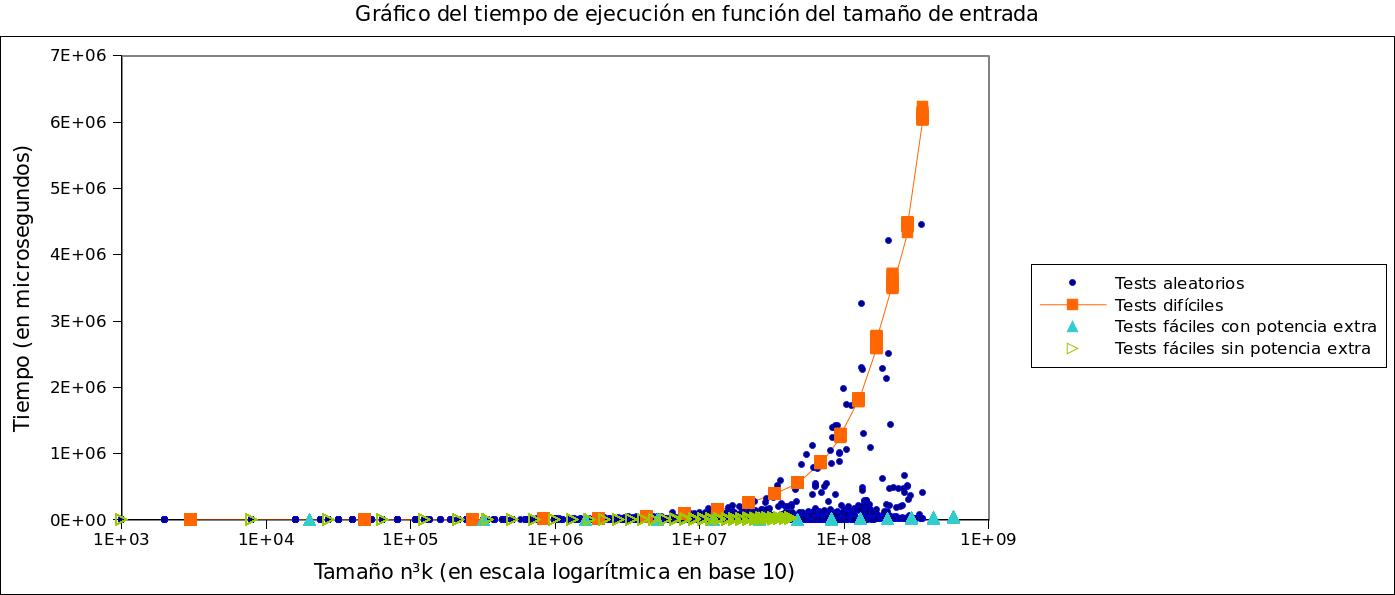
\includegraphics[width=\textwidth]{Grafico1.jpg}

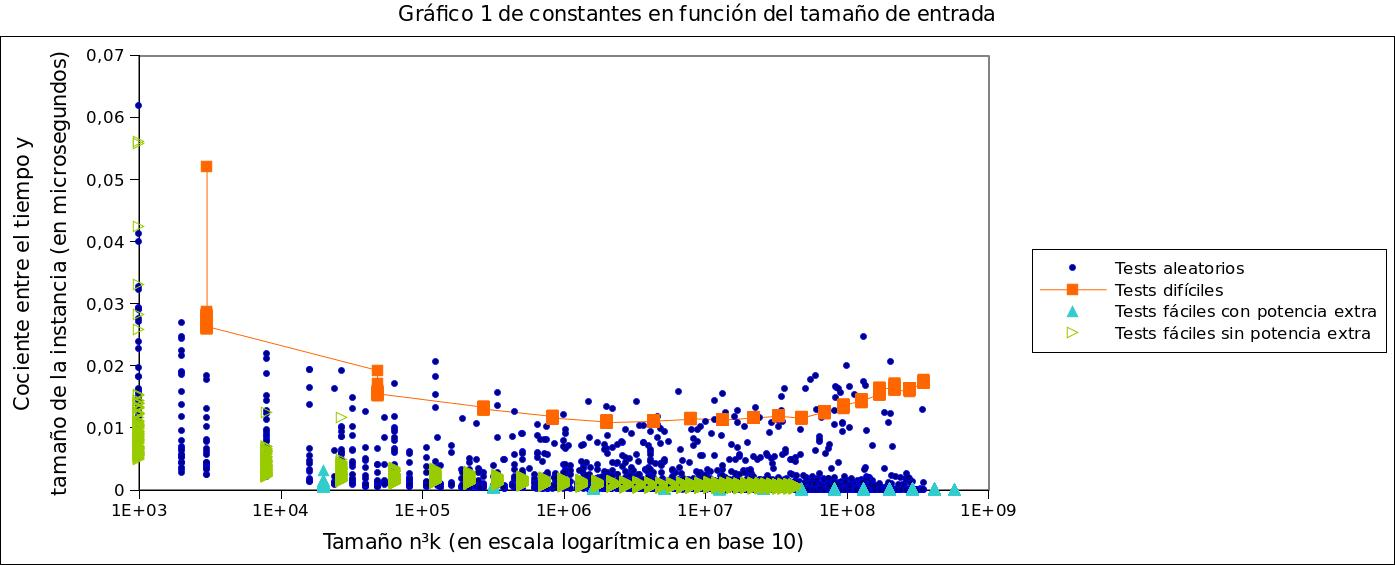
\includegraphics[width=\textwidth]{Grafico2.jpg}

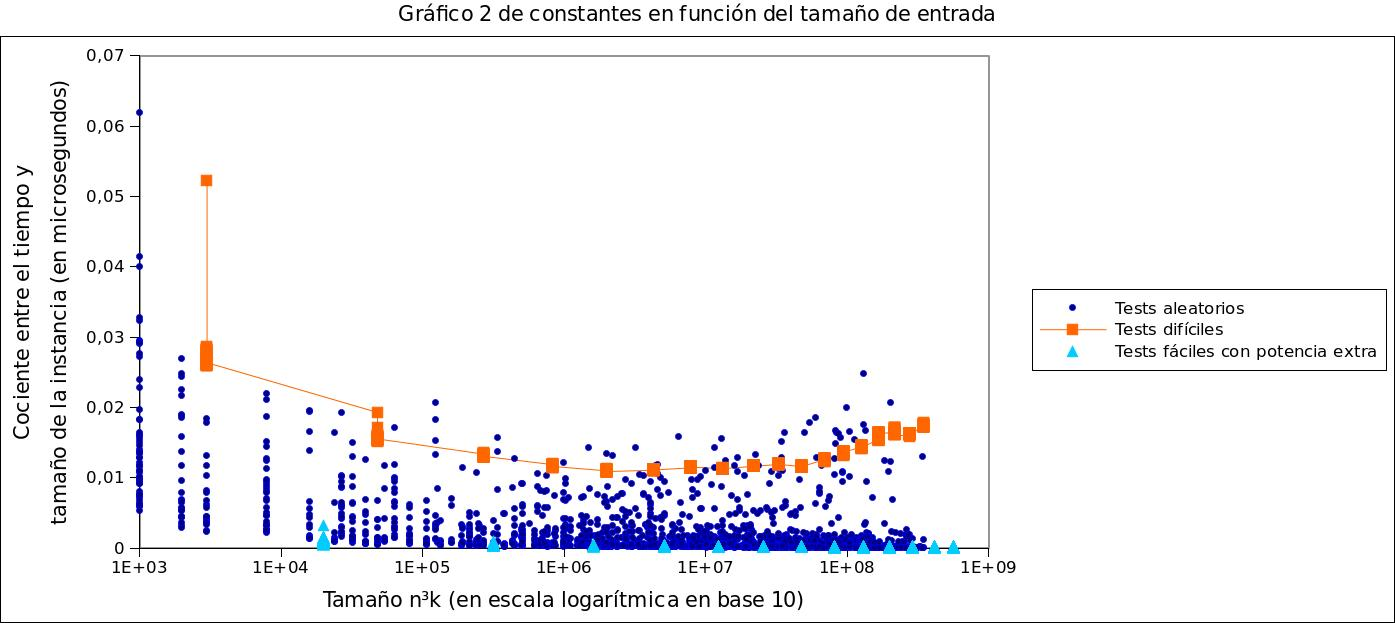
\includegraphics[width=\textwidth]{Grafico3.jpg}

\subsubsection{Conclusiones}

Como se puede ver en el segundo y tercer gr�fico, los tests dif�ciles no son los de caso peor, pero a�n as� se disponen en una constante.
Hay \textit{outliers} para cada tanda de instancias, que son m�s notorios para $n^3*k$ chicos. Estos surgen por ser las primeras mediciones de una instancia del programa. Como est� obteniendo las variables en memoria por primera vez, hay valores que faltan en la memoria cache del procesador. Posteriormente desaparecen del gr�fico los \textit{outliers} porque es un costo constante.



\subsection{Desarrollo de los ejercicios adicionales}

\begin{enumerate} 
\item El algoritmo de creaci�n de la matriz permanecer�a pr�cticamente igual, las aristas ahora tienen peso $d*c(r)$, donde $c(r)$ es el costo asociado
a cada resorte, y $d$ es la distancia a saltar. Sin embargo, si utilizamos unidades de potencia para realizar los saltos, esto es modelado con otro conjunto de aristas,
las cuales tienen peso $(d-i)*c(r)$, con $1 \leq i \leq k$. Esto representa el hecho de saltar utilizando $1,2,...,k$ unidades de potencia.
Una gran diferencia con el algoritmo anterior es que si un salto se pod�a hacer sin gastar potencia extra entonces no nos interesaba el mismo salto gastando potencia extra.
Esto significa que al generar las aristas por cada v�rtice tenemos, siendo $n$ la cantidad de v�rtices, en el peor caso $2n*k$ aristas, donde antes ten�amos $2n$ aristas. (Nos podr�a interesar gastar $k$ en vez de dinero pues lo que estamos minimizando es el dinero gastado). 
Entonces, ahora nuestro modelo tiene aristas de peso positivo, con pesos no necesariamente iguales. Por lo tanto, para resolver el problema, utilizamos el 
algoritmo de Dijkstra, ya que se cumple que el grafo no tiene pesos negativos, y al ser los pesos distintos, no podemos utilizar algoritmos m�s eficientes como BFS.


\item La complejidad del algoritmo se divide en dos partes: crear el grafo con las caracter�sticas mencionadas, y aplicarle al grafo el algoritmo de Dijkstra. La construcci�n de este nuevo grafo var�a su complejidad respecto del problema original debido a que ponerle peso a las aristas es $O(1)$, pero la cantidad de aristas por cada v�rtice se multiplica por $k$. %COMENTARIO: VER SI SE DUPLICAN LAS ARISTAS.
Luego, aplicar el algoritmo de Dijkstra cuesta $O(m*log(n))$, siendo $m$ la cantidad de aristas. Como el grafo tiene un tama�o de $n^2*k$, y cada v�rtice se puede conectar con $2n*k$ otros v�rtices en el peor caso
entonces $m = (2n*k)*(n^2*k)$. Luego Dijkstra cuesta $O(n^3*k^2*log(n^2*k))$.
La complejidad de utilizar Dijkstra es mayor que la de crear el grafo, por lo tanto la complejidad final ser�a $O(n^3*k^2*log(n^3*k^2))$.
\end{enumerate} 


%\newpage
%\section{Ap�ndice I: C�digo fuente}
%
%
\subsection{C�digo fuente del problema 1}

\subsection{C�digo fuente del problema 2}

\newpage
\subsection{C�digo fuente del problema 3}

	\subsubsection{problema3.h}

	\begin{small}
		\lstinputlisting{ej3/problema3.h}
	\end{small}
	%\newpage

	\subsubsection{problema3.cpp}

	\begin{small}
		\lstinputlisting{ej3/problema3.cpp}
	\end{small}
	%\newpage

	\subsubsection{matrix.h}

	\begin{small}
		\lstinputlisting{ej3/matrix.h}
	\end{small}
	%\newpage

	\subsubsection{matrix.cpp}

	\begin{small}
		\lstinputlisting{ej3/matrix.cpp}
	\end{small}
	%\newpage

	\subsubsection{latablita.h}

	\begin{small}
		\lstinputlisting{ej3/latablita.h}
	\end{small}
	%\newpage

	\subsubsection{latablita.cpp}

	\begin{small}
		\lstinputlisting{ej3/latablita.cpp}
	\end{small}
	%\newpage

	\subsubsection{caminomin.h}

	\begin{small}
		\lstinputlisting{ej3/caminomin.h}
	\end{small}
	%\newpage

	\subsubsection{caminomin.cpp}

	\begin{small}
		\lstinputlisting{ej3/caminomin.cpp}
	\end{small}
	%\newpage

	\subsubsection{tipos.h}

	\begin{small}
		\lstinputlisting{ej3/tipos.h}
	\end{small}

\end{document}
